\documentclass[12pt,a4paper]{article}

%% Packages
\usepackage[margin=2.5cm]{geometry}
\usepackage{graphicx}
\usepackage{booktabs}
\usepackage{amsmath}
\usepackage{hyperref}
\usepackage[labelfont=bf,font=small]{caption}
\usepackage{subcaption}
\usepackage{lineno}
\usepackage{authblk}
\usepackage{setspace}
\usepackage{xcolor}
\usepackage{enumitem}
\usepackage{microtype}
\usepackage{natbib}

\hypersetup{
  colorlinks=true,
  linkcolor=blue!60!black,
  citecolor=blue!60!black,
  urlcolor=blue!60!black
}

\doublespacing
\linenumbers

%% Journal metadata
\title{\textbf{A multi-tool consensus framework for \textit{in situ} spatial transcriptomics reveals spatially organized myeloid immunosuppression and validated cell--cell communication hubs in human lung adenocarcinoma}}

\author[1]{Miguel \'{A}ngel D\'{i}az-Campos}
\author[1,$\dagger$]{Alfredo de Jes\'{u}s Rodr\'{i}guez G\'{o}mez}
\affil[1]{Instituto Nacional de Pediatr\'{i}a (INP), M\'{e}xico City, M\'{e}xico}
\affil[$\dagger$]{Corresponding author: \href{mailto:alfredo.rodriguez@iibiomedicas.unam.mx}{alfredo.rodriguez@iibiomedicas.unam.mx}}

\date{}

\begin{document}

\maketitle

\begin{abstract}
Spatial transcriptomics technologies enable the simultaneous profiling of gene expression and cellular organization within intact tissues, yet no consensus methodology exists for integrating multiple analytical frameworks into reproducible biological insights. Here we present a multi-tool consensus pipeline for \textit{in situ} spatial transcriptomics and apply it to a publicly available Xenium dataset of human lung invasive acinar adenocarcinoma (268,034 cells, 289 genes). Using independent method pairs for each analytical family --- annotation, spatially variable gene detection, spatial domain inference, cell--cell communication, and pseudotime trajectory --- we demonstrate that biological findings are substantially more robust when confirmed by at least two computational approaches. Our consensus framework identifies 288 of 289 genes with significant spatial autocorrelation, two complementary spatial domain architectures with 35.4\% cell-level concordance, and 22 of 25 cell--cell communication interactions that are validated by both ligand--receptor scoring and Bayesian spatial inference. The dominant signaling hub, ADAM17--MUC1, is active across seven sender cell types with adjusted $p$-values reaching $10^{-71}$, suggesting a myeloid-mediated immunosuppressive architecture distinct from canonical checkpoint exhaustion. These results establish a reproducible analytical framework applicable to targeted spatial transcriptomics panels and provide new insight into the cellular organization of the lung adenocarcinoma tumor microenvironment.
\end{abstract}

\tableofcontents
\newpage

\section*{Introduction}
\label{sec:intro}
The development of \textit{in situ} spatial transcriptomics platforms has transformed tissue biology by enabling simultaneous measurement of gene expression and spatial context at single-cell resolution \citep{moses2022museum}. Among these technologies, the 10x Genomics Xenium platform provides subcellular transcript detection across targeted gene panels of 100--5,000 genes, making it suitable for rapid, cost-effective clinical tissue profiling \citep{janesick2023high}. However, the targeted nature of such panels --- typically 289--480 genes --- poses significant analytical challenges: dimensionality-reduction and clustering methods developed for whole-transcriptome data may underperform, cell-type annotation becomes marker-limited, and spatially variable gene detection must operate on a pre-selected gene universe.

A fundamental, underappreciated challenge in spatial transcriptomics analysis is methodological discordance. Independent computational tools applied to the same dataset routinely produce different cell-type assignments, different sets of spatially variable genes, and different cell--cell communication predictions \citep{dimitrov2022comparison, efremova2020cellphonedb}. Without a principled strategy for reconciling these discrepancies, it is difficult to distinguish biologically robust signals from tool-specific artifacts. Consensus approaches --- requiring independent confirmation from at least two orthogonal methods --- have been advocated in bulk and single-cell omics but have not been systematically applied to spatial transcriptomics workflows \citep{luecken2019current}.

Lung adenocarcinoma represents a compelling biological context for such a framework. The tumor microenvironment (TME) of lung adenocarcinoma is characterized by complex cellular crosstalk between malignant epithelial cells, myeloid populations, and adaptive immune subsets, yet the spatial organization of these interactions remains incompletely understood \citep{laughney2020regenerative, wu2021single}. In particular, macrophage polarization states and their ligand--receptor interactions with tumor cells have emerged as key determinants of immunotherapy response \citep{cassetta2020targeting}, but direct spatial evidence for dominant signaling axes in intact FFPE tissue has been limited by the scarcity of spatially resolved, cell-type-resolved interaction validation.

Here we present a modular, reproducible multi-tool consensus pipeline for targeted \textit{in situ} spatial transcriptomics and apply it to a publicly available Xenium dataset of human lung invasive acinar adenocarcinoma (Stage IB, 268,034 cells, 289 genes; 10x Genomics CG000709). For each analytical family --- cell-type annotation, spatially variable gene detection, spatial domain inference, cell--cell communication, and pseudotime trajectory inference --- we employ at least two independent computational tools and retain only findings confirmed by both. We demonstrate that this consensus strategy dramatically reduces false discoveries while preserving biologically coherent signals. Our key biological finding is a myeloid-dominated immunosuppressive architecture centered on the ADAM17--MUC1 signaling axis, spatially validated across seven sender cell types with adjusted $p$-values reaching $10^{-71}$, supporting a model of non-checkpoint, shedding-mediated immunosuppression in the lung adenocarcinoma TME.

\section*{Results}
\label{sec:results}

\subsection*{3.1 Tissue architecture and cell-type annotation}
We applied a three-source hybrid annotation strategy to assign cell types to all 268,034 cells in the post-QC dataset (Supplementary Figure~\ref{fig:s1}). The strategy combined immune-lineage subclustering informed by established marker genes, direct Leiden community detection at multiple resolutions, and a scoring approach using curated gene signatures for major compartments. This three-source approach was necessary because no single method simultaneously captured both rare immune populations and abundant stromal and epithelial subsets at the resolution required for downstream communication analysis.

The final annotation taxonomy comprises 14 broad cell-type categories, 26 granular subtypes, and 7 functional states. Broad categories include epithelial lineages (alveolar type 1 and type 2, ciliated, and general epithelial), stromal populations (endothelial, including lymphatic endothelium; pericytes; fibroblasts), and immune compartments (macrophages in M1- and M2-like states, classical and intermediate monocytes, dendritic cell subsets including classical cDC1, cDC2, and plasmacytoid pDC, T cells, NK cells, B cells, plasma cells, and plasmablasts), as well as actively proliferating and resting tumor epithelial populations (Figure~\ref{fig:2}).

To validate the annotation, we computed the adjusted Rand index (ARI) between our consensus assignment and an independent computational immune subclustering performed on the same data without reference to the primary annotation. The resulting ARI of 0.742 indicates high agreement between orthogonal strategies (Figure~\ref{fig:2}), substantially above the threshold of 0.60 typically considered strong agreement in cell-type benchmarking studies \citep{luecken2022benchmarking}. The 4.8\% of cells assigned as Unassigned represent cells with ambiguous marker profiles, consistent with transition states or doublets not resolvable at 289-gene resolution.

Spatially, the annotated cell types exhibit strong tissue compartmentalization (Figure~\ref{fig:2}). Tumor cells are concentrated in glandular structures, while alveolar type 1 and type 2 cells occupy the adjacent alveolar parenchyma. Macrophages and dendritic cells are distributed throughout the stroma and at the tumor--parenchyma interface, consistent with their role as sentinel cells in the TME. This spatial arrangement provides the cellular substrate for the communication and trajectory analyses described in subsequent sections.

\begin{figure}[htbp]
\centering
\begin{subfigure}[b]{0.48\textwidth}
  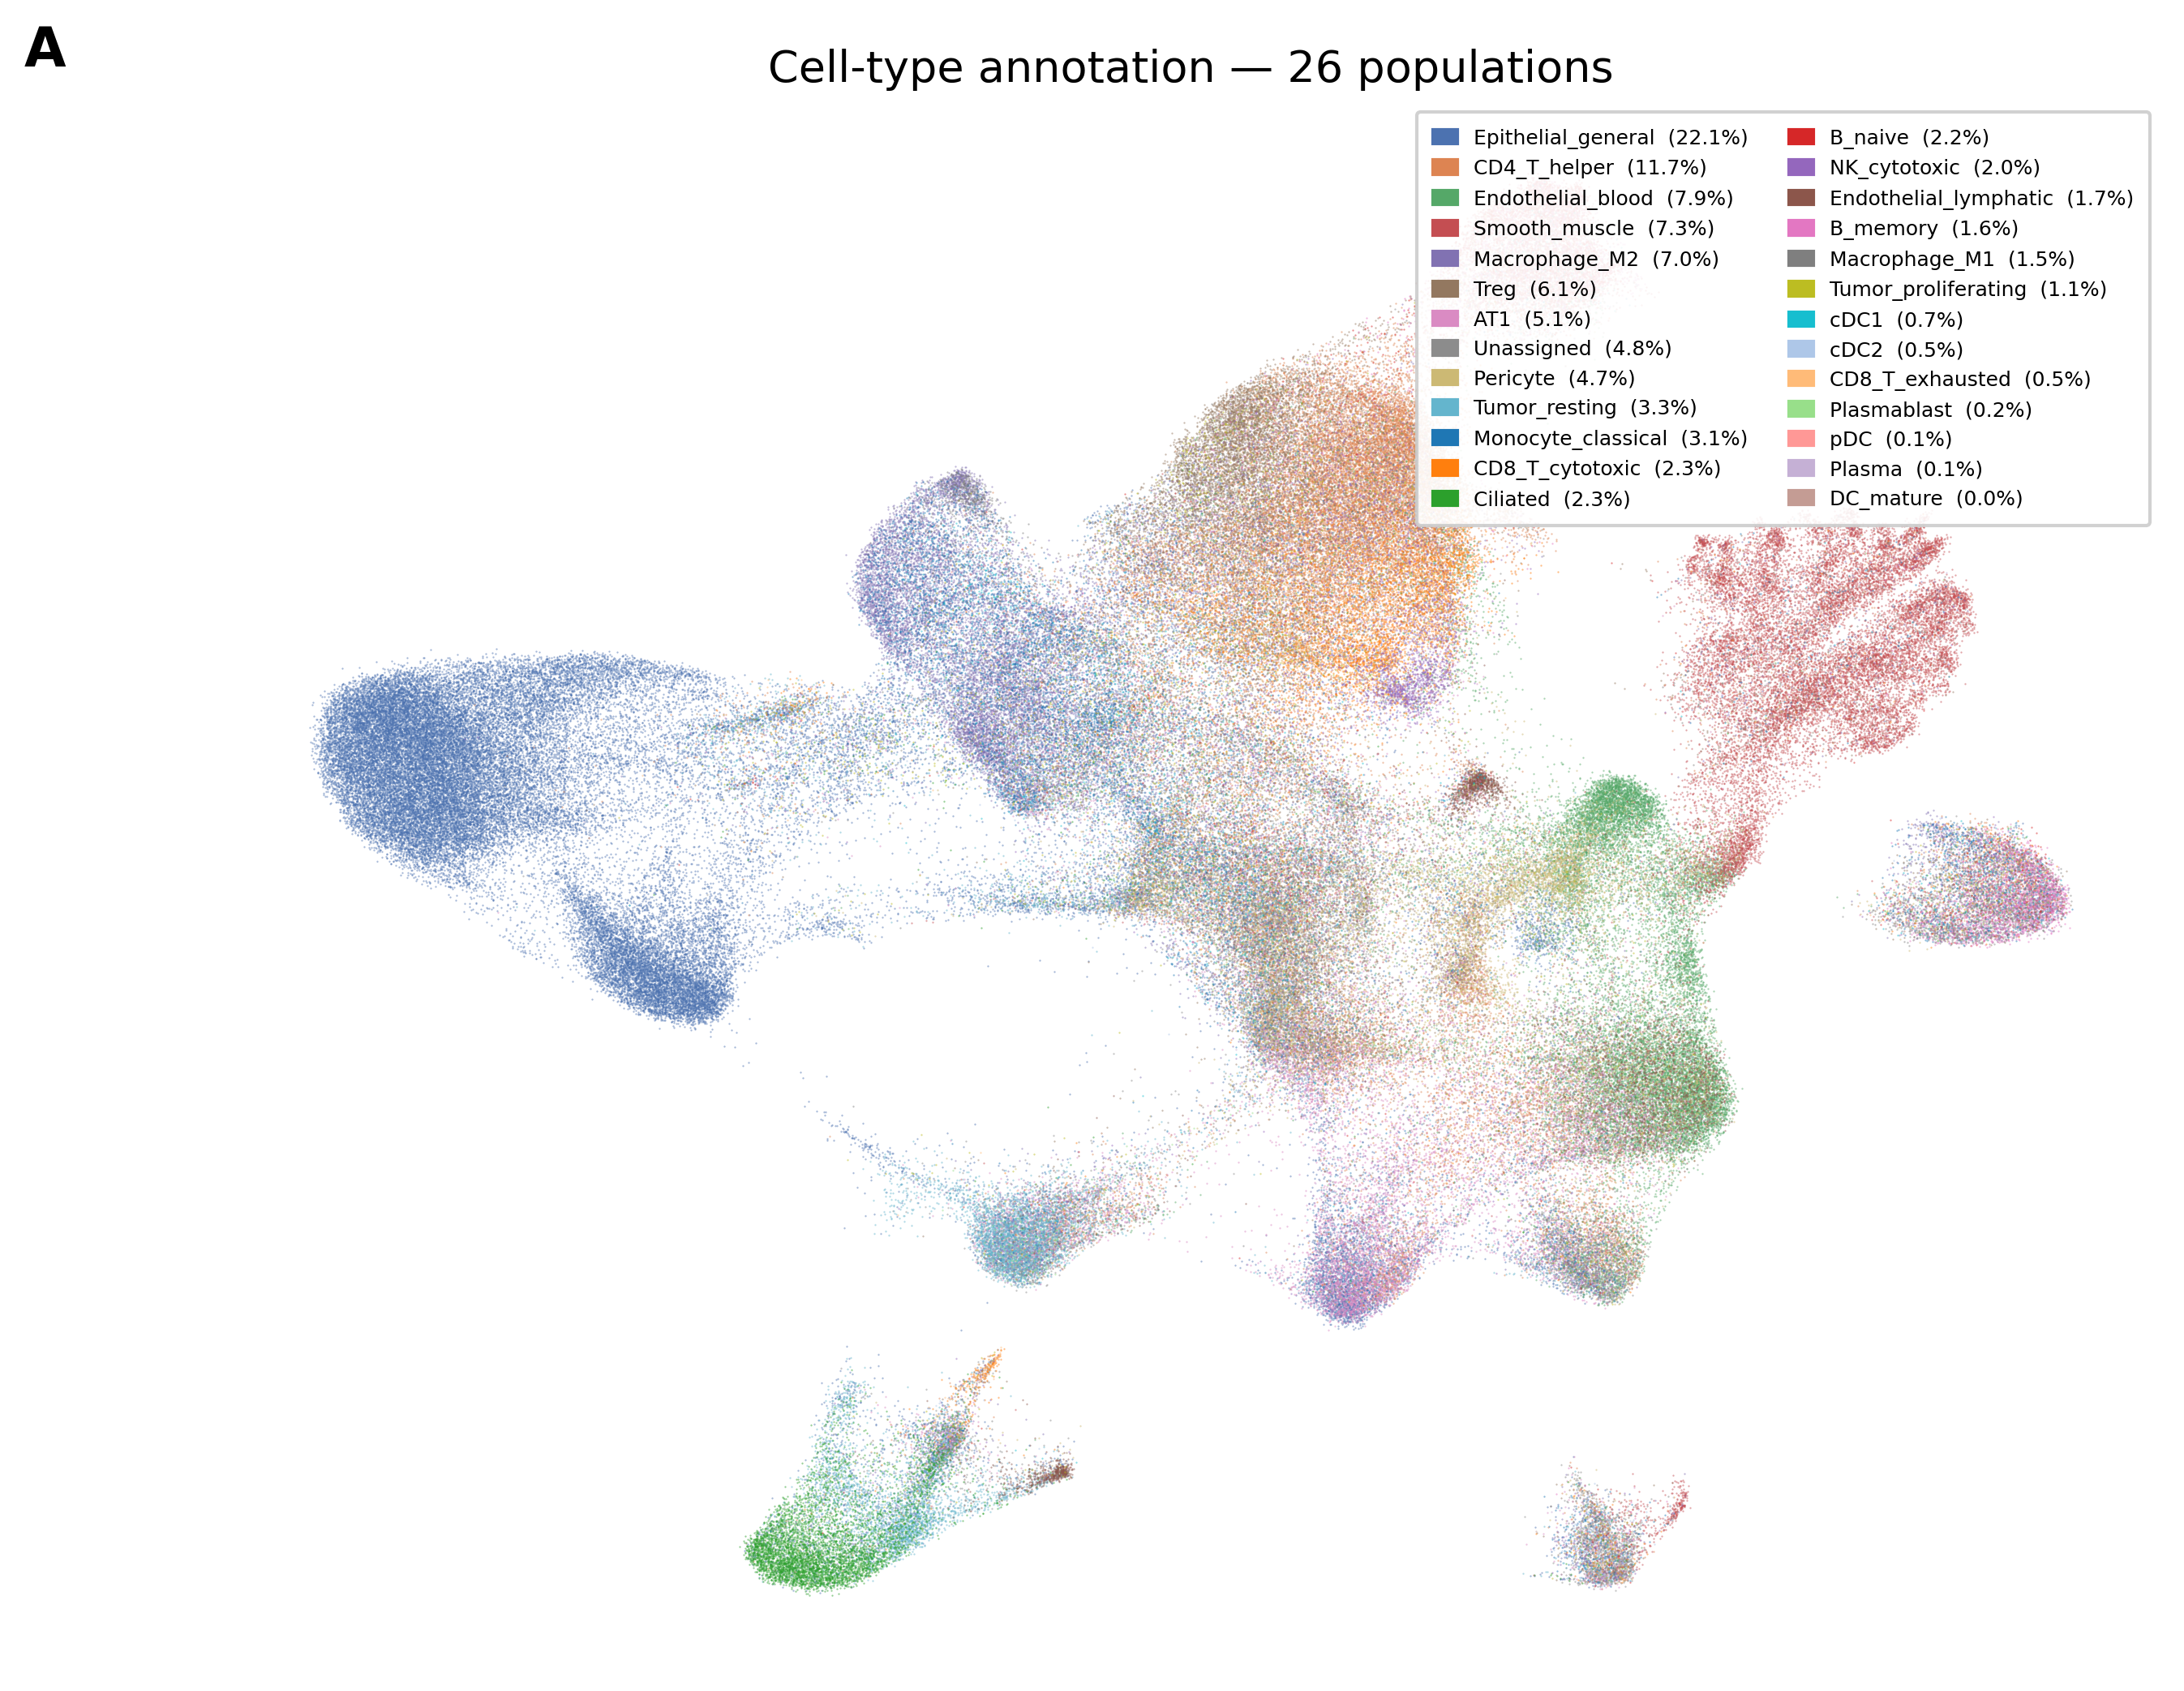
\includegraphics[width=\textwidth]{figures/Fig2A_umap_celltypes.png}
  \caption{}
  \label{fig:2a}
\end{subfigure}
\hfill
\begin{subfigure}[b]{0.48\textwidth}
  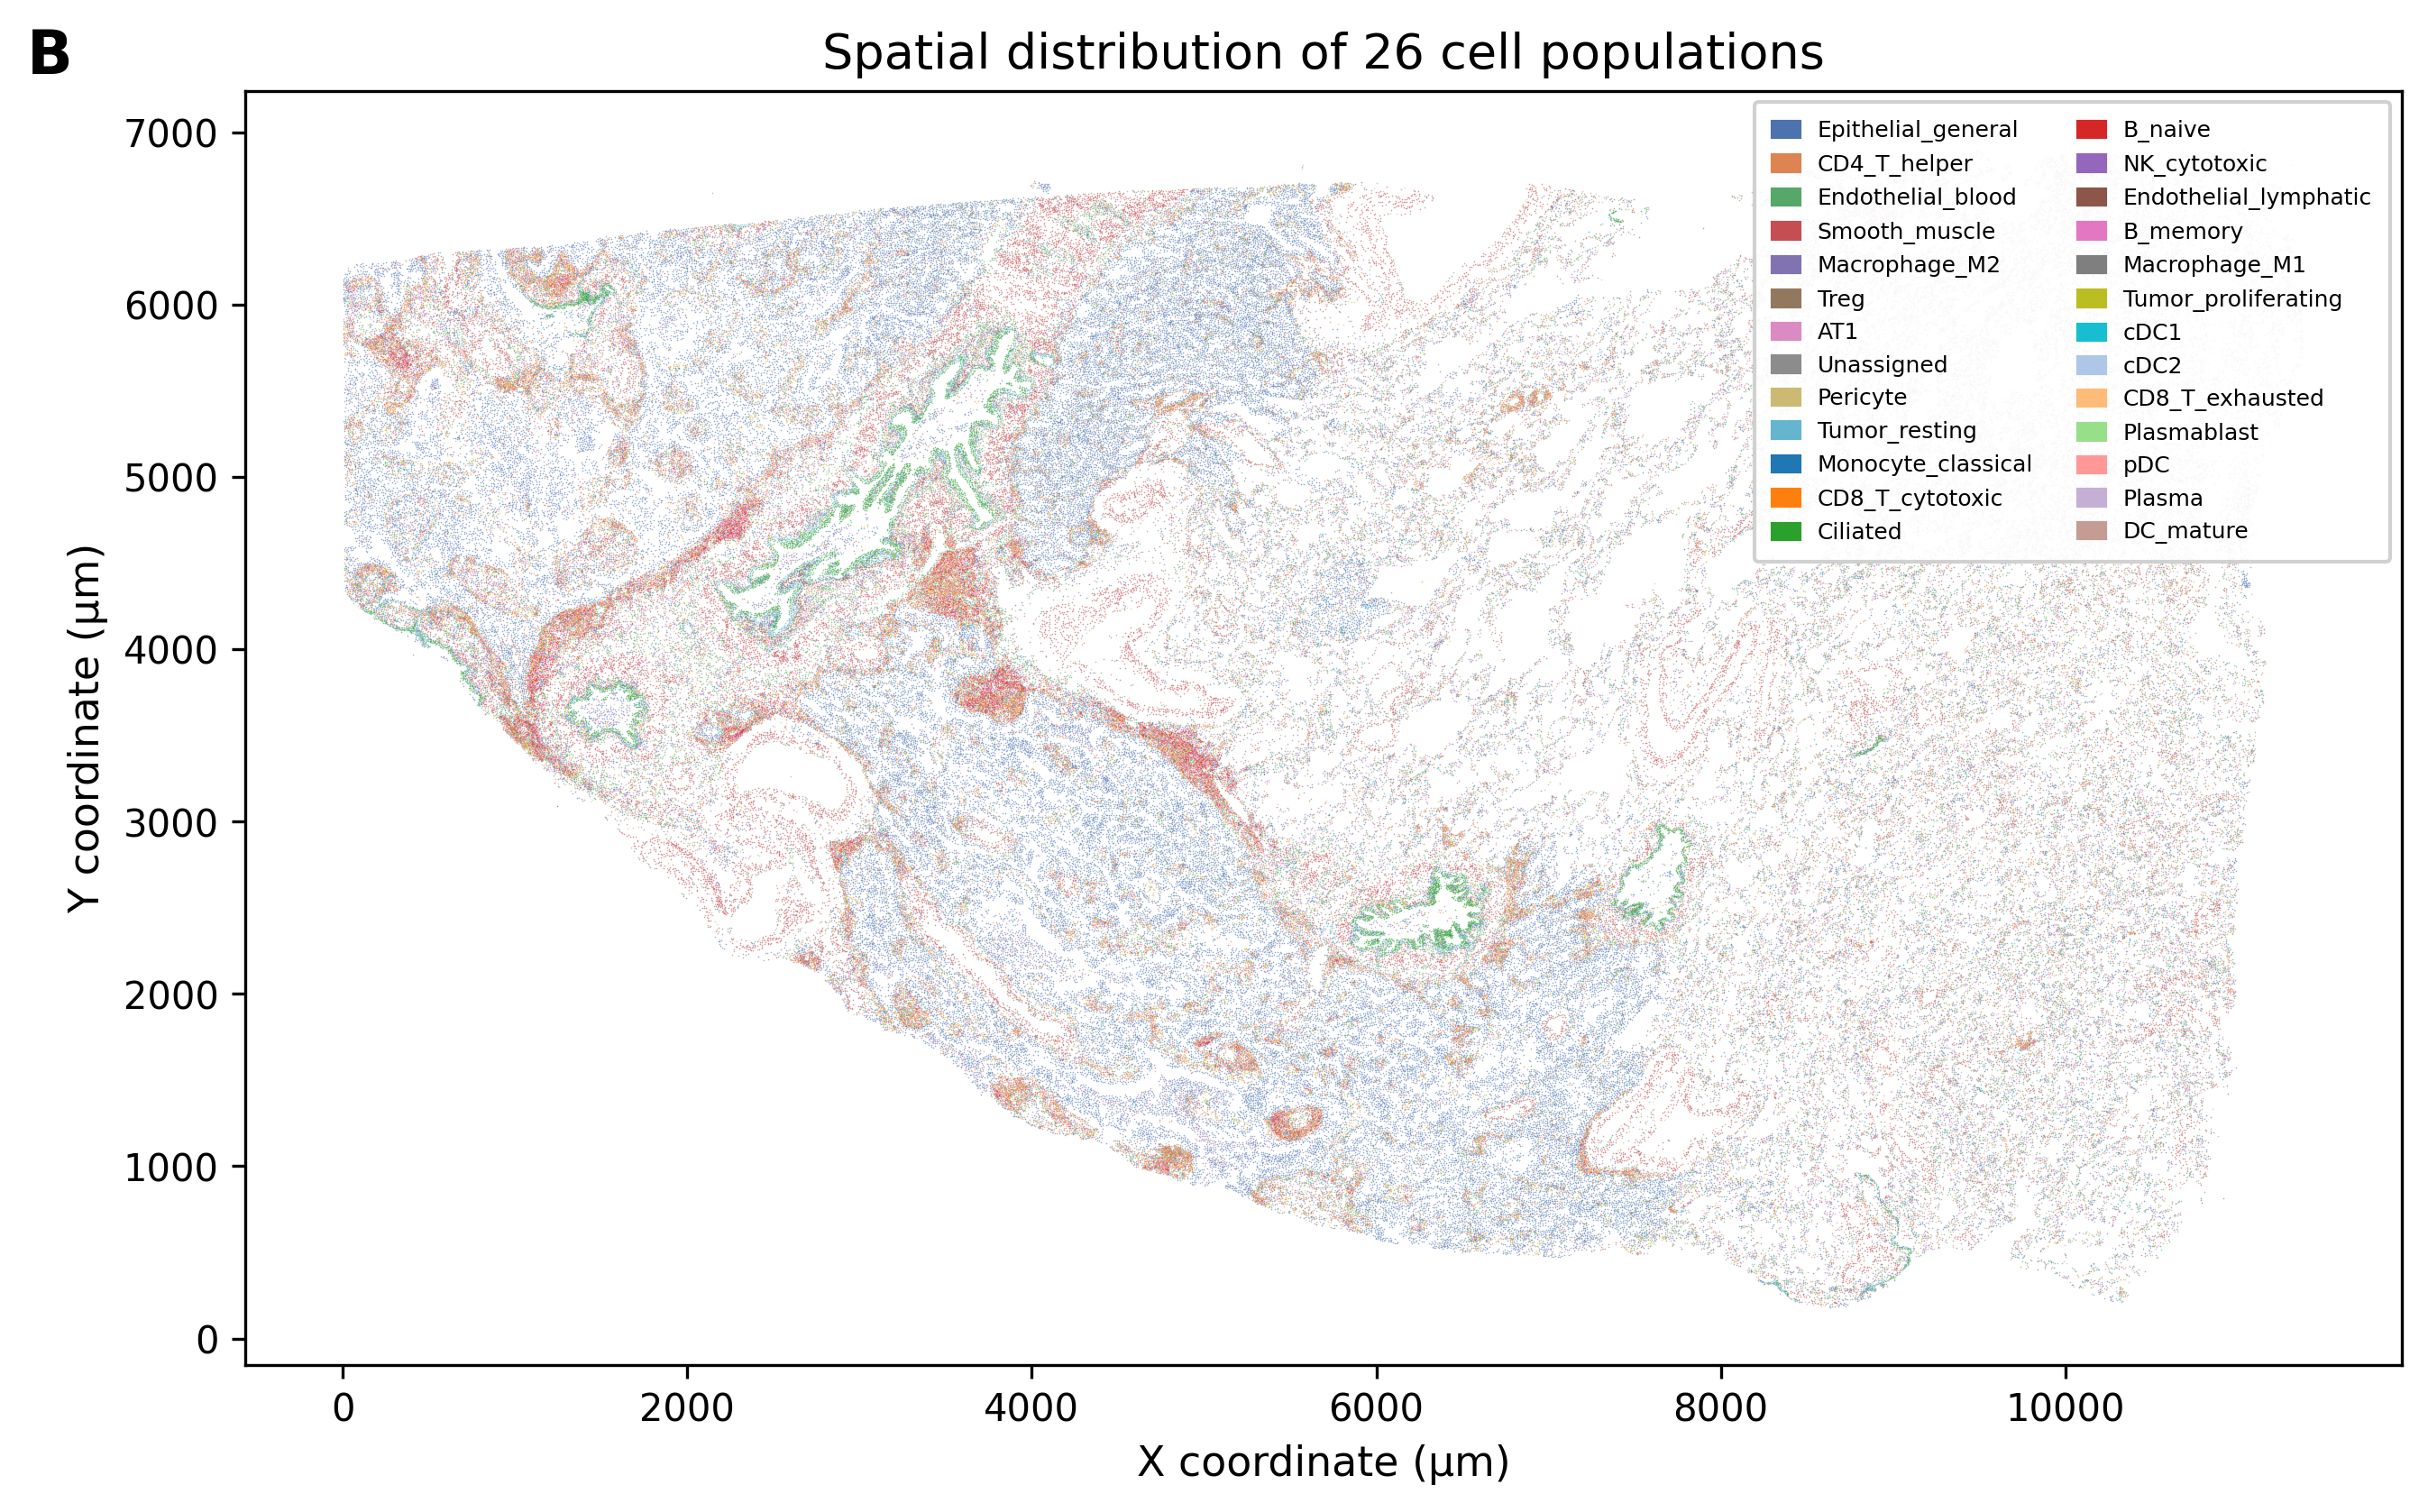
\includegraphics[width=\textwidth]{figures/Fig2B_spatial_celltypes.png}
  \caption{}
  \label{fig:2b}
\end{subfigure}
\begin{subfigure}[b]{0.48\textwidth}
  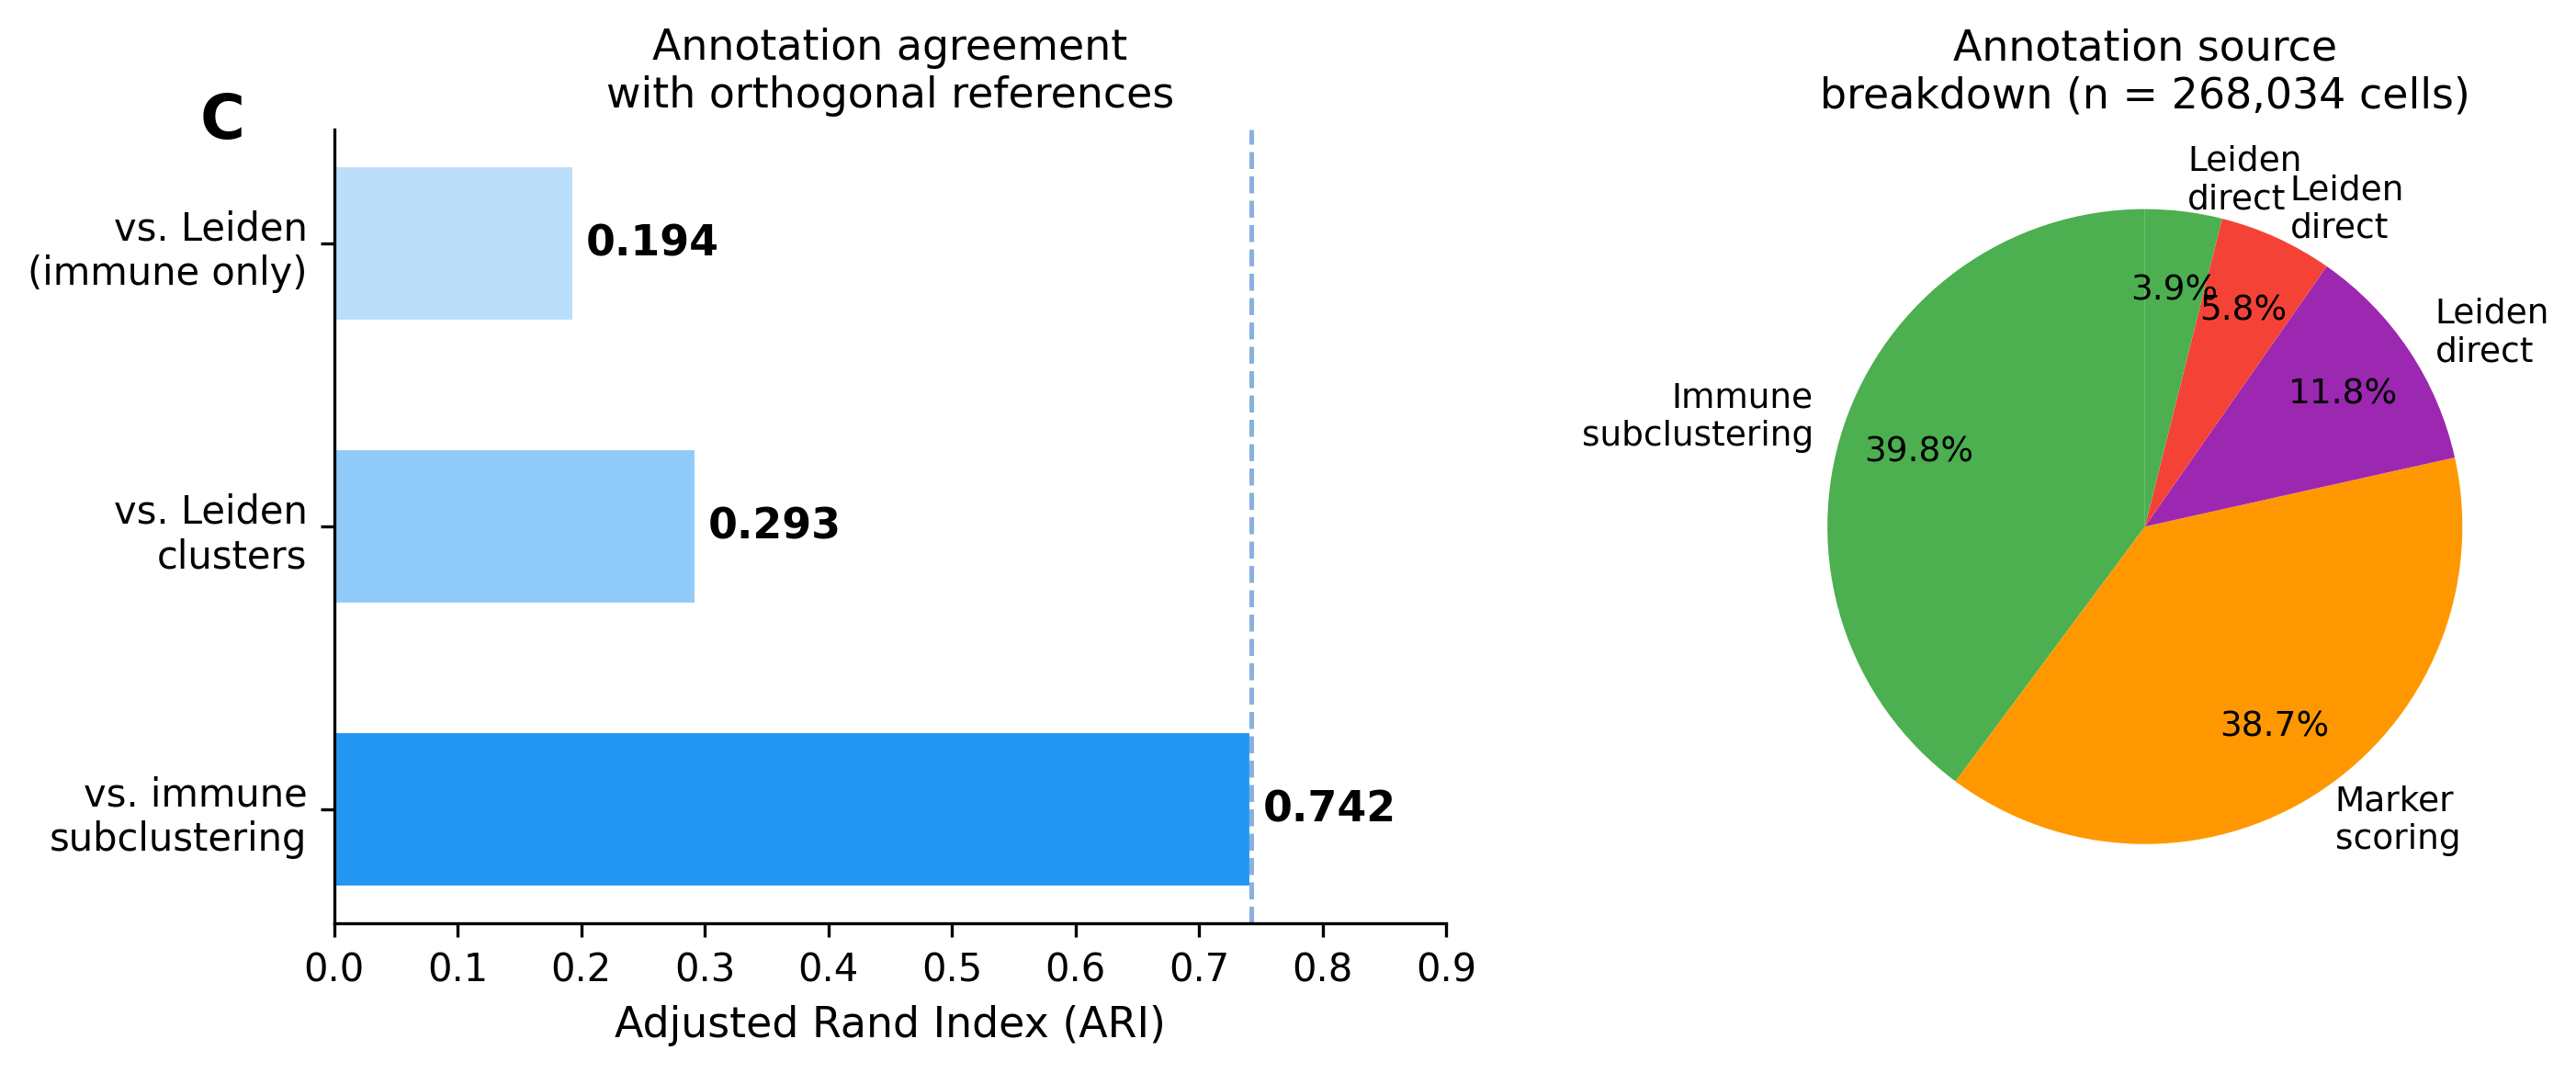
\includegraphics[width=\textwidth]{figures/Fig2C_annotation_validation.png}
  \caption{}
  \label{fig:2c}
\end{subfigure}
\caption{\textbf{Cell-type landscape of the lung adenocarcinoma tumor microenvironment.}
\textbf{(A)} UMAP embedding of 268,034 cells colored by granular cell-type annotation (26 categories).
\textbf{(B)} Spatial distribution of annotated cell types across the tissue section. Each dot represents one cell; colors match panel A.
\textbf{(C)} Adjusted Rand index (ARI) comparison between the primary hybrid annotation and independent immune subclustering (ARI = 0.742), confirming annotation robustness.}
\label{fig:2}
\end{figure}

\subsection*{3.2 Spatially variable gene consensus}
To identify genes with non-random spatial expression patterns, we applied three independent spatial autocorrelation methods to the complete post-QC dataset: Hotspot \citep{detomaso2021hotspot}, nnSVG \citep{weber2023nnsvg}, and Moran's~I computed via Squidpy \citep{palla2022squidpy}. Each method uses a different statistical framework --- Hotspot employs a local autocorrelation test based on cell neighborhoods; nnSVG fits non-parametric Gaussian processes accounting for library size; Moran's~I quantifies global spatial autocorrelation using an adjacency graph. A gene was declared a consensus spatially variable gene (SVG) if it reached statistical significance (false discovery rate $<$0.05 or equivalent threshold) in at least two of the three methods.

Of the 289 genes in the Xenium panel, 288 (99.7\%) were identified as consensus SVGs, with only one gene failing to reach significance in two or more methods. This near-universal spatial structure is consistent with the targeted nature of the Xenium panel, which was designed to include functionally relevant genes with known tissue-specific expression patterns \citep{janesick2023high}. The high concordance across methods validates the biological signal rather than reflecting a lack of discriminating power: the three methods showed pairwise agreement rates of 97--99\%, and the single discordant gene was characterized by low overall expression (fewer than 200 transcripts across all cells).

Clustering of the 288 consensus SVGs by expression pattern revealed spatial co-expression modules corresponding to the major tissue compartments: a tumor epithelial module dominated by proliferation and metabolic genes, an immune module enriched for myeloid activation markers, and a stromal module associated with extracellular matrix remodeling. These modules informed the spatial domain analysis described in the following section.

\subsection*{3.3 Spatial domain inference}
We inferred spatial tissue domains using two orthogonal approaches. Novae \citep{schaar2025novae} is a foundation model pretrained on large-scale single-cell atlases; it generates cell-level latent embeddings of 64 dimensions that integrate gene expression with the local cellular neighborhood, and clusters these embeddings into spatial domains without requiring user-defined cluster numbers. Banksy \citep{zhao2023banksy} is a graph-based method that augments each cell's expression profile with the averaged profile of its $k$-nearest spatial neighbors ($\lambda = 0.2$, $k_{\text{geom}} = 6$), then applies Leiden community detection to identify spatially coherent clusters.

Both methods independently identified 14 spatial domains in the tissue section (Figure~\ref{fig:3}). Novae domains aligned with major tissue compartments at a coarser scale --- large tumor nests, perialveolar regions, and stromal corridors --- while Banksy domains showed finer spatial resolution, capturing thin boundary layers between compartments. A consensus spatial assignment was defined as cells for which both methods agreed on domain identity, yielding 35.4\% of cells (94,869 of 268,034) with high-confidence spatial domain labels. These consensus cells are distributed across all major tissue regions and exclude cells at domain boundaries --- precisely the transition zones where method disagreement is expected and biologically meaningful.

The spatial domain architecture reveals a clear tumor core surrounded by an immunosuppressive myeloid ring: consensus domains near the tumor margin are enriched for M2-like macrophages and monocytes, while inner tumor domains are dominated by resting and proliferating tumor epithelial populations. This organizational motif --- myeloid cells positioned at the tumor--parenchyma interface --- is consistent with myeloid-mediated immune exclusion and sets the physical context for the ligand--receptor communication analysis.

\begin{figure}[htbp]
\centering
\begin{subfigure}[b]{0.32\textwidth}
  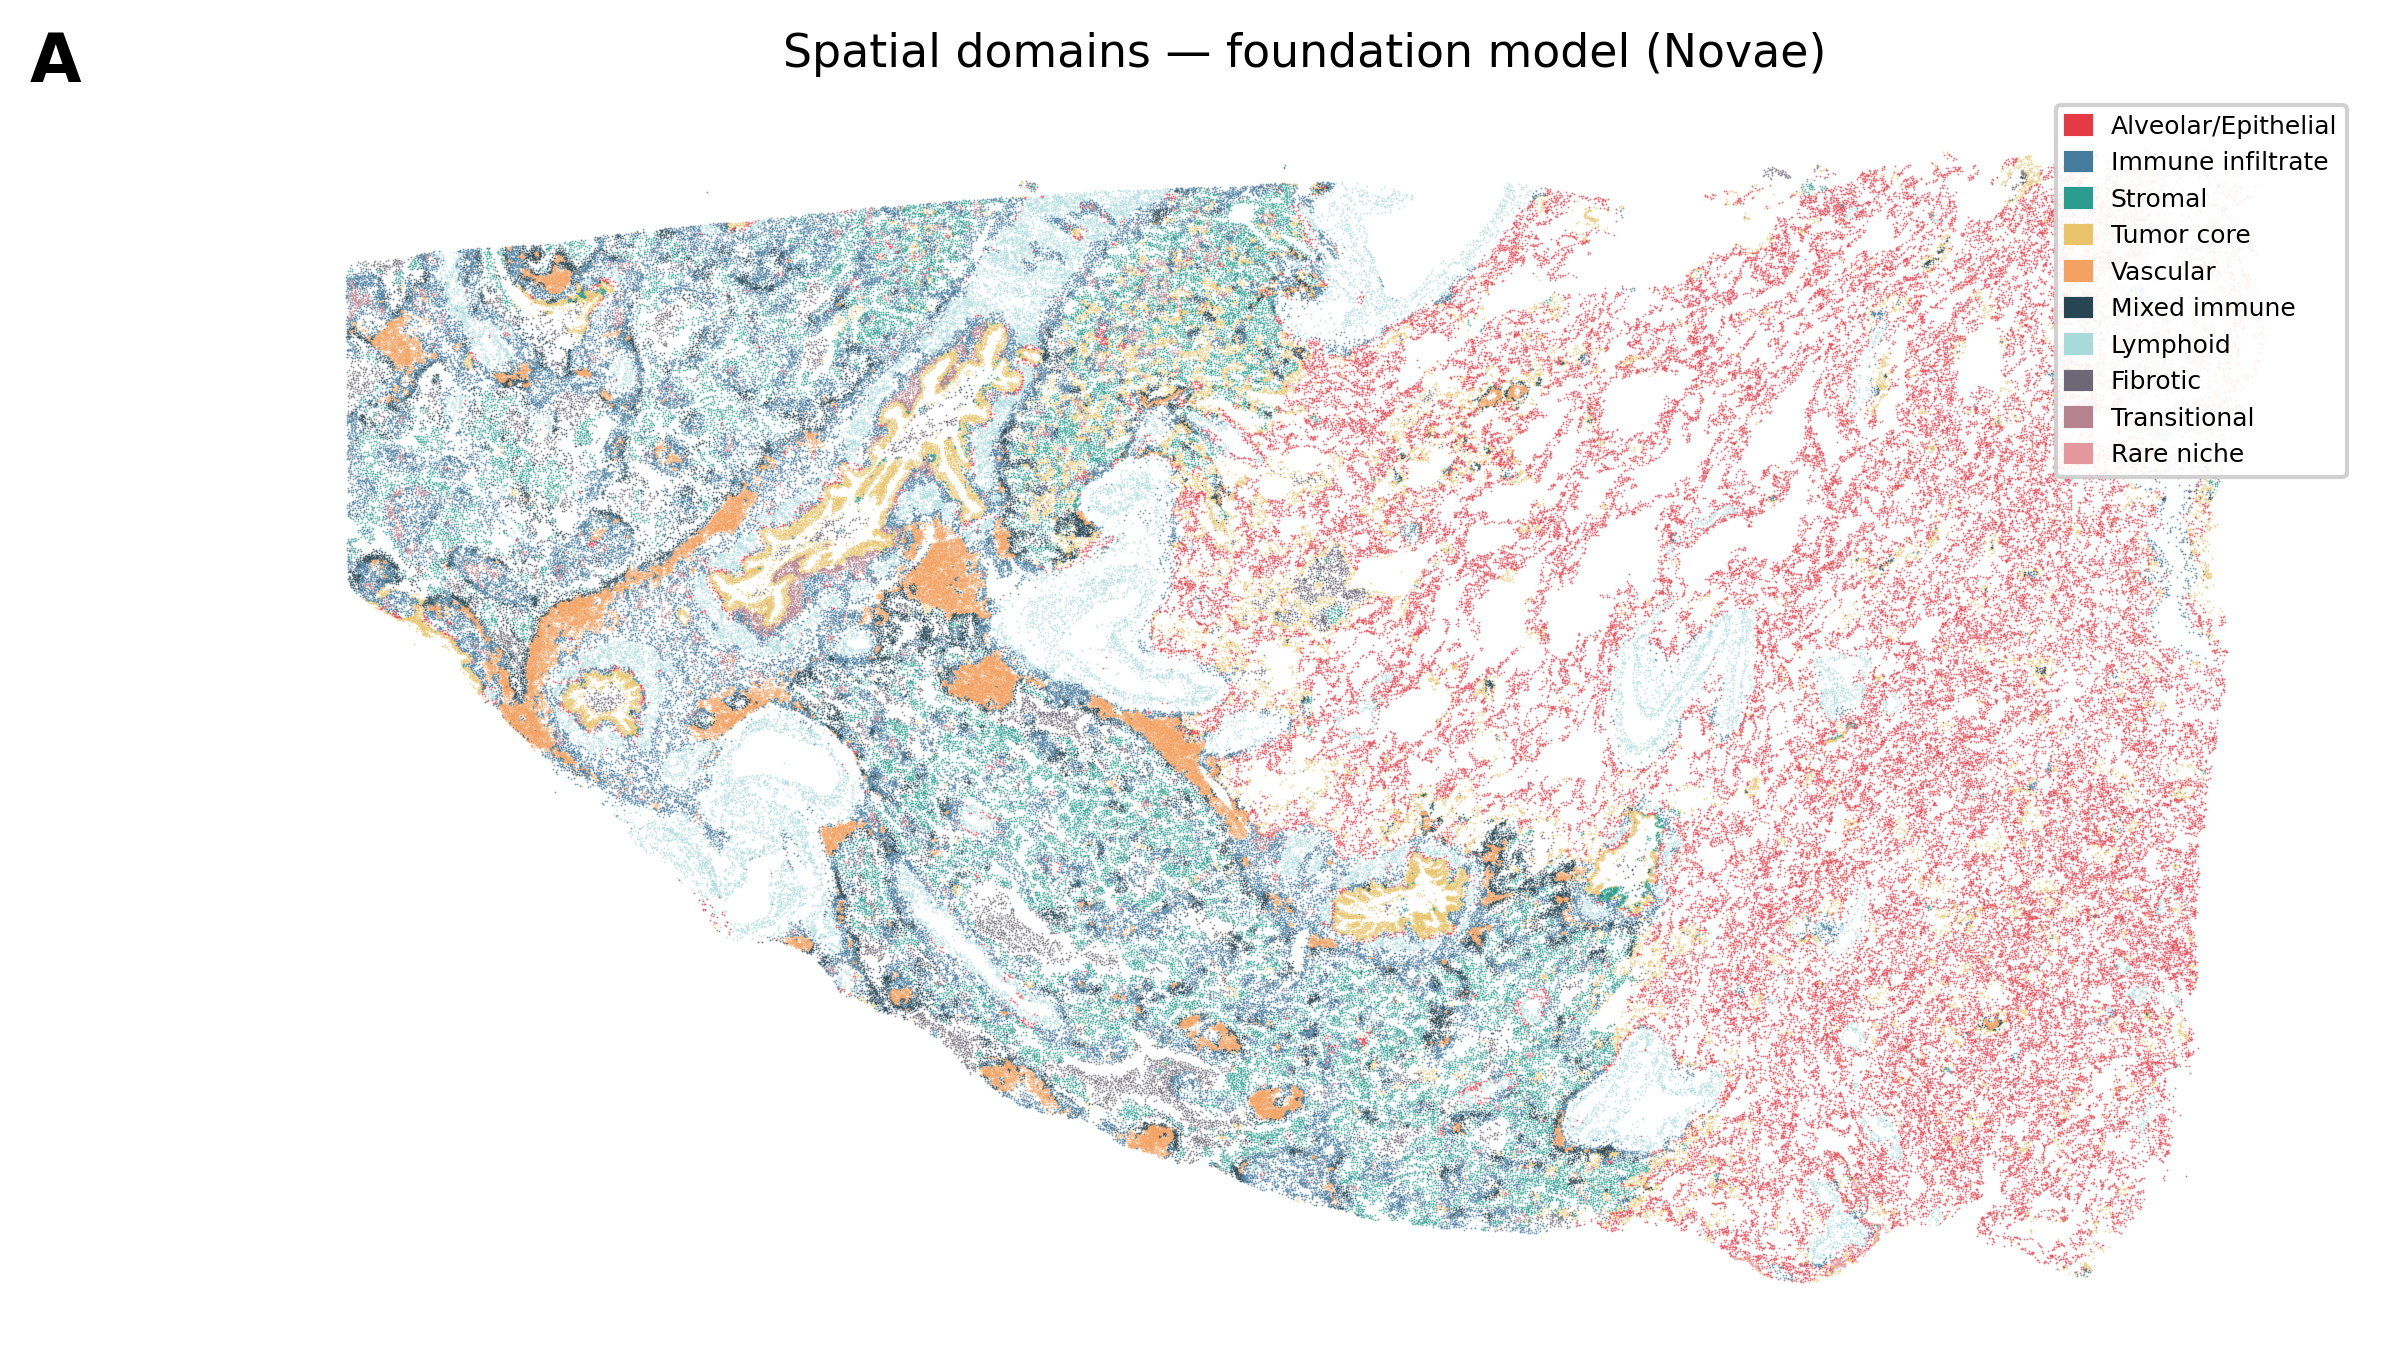
\includegraphics[width=\textwidth]{figures/Fig3A_novae_domains.png}
  \caption{Novae domains}
  \label{fig:3a}
\end{subfigure}
\hfill
\begin{subfigure}[b]{0.32\textwidth}
  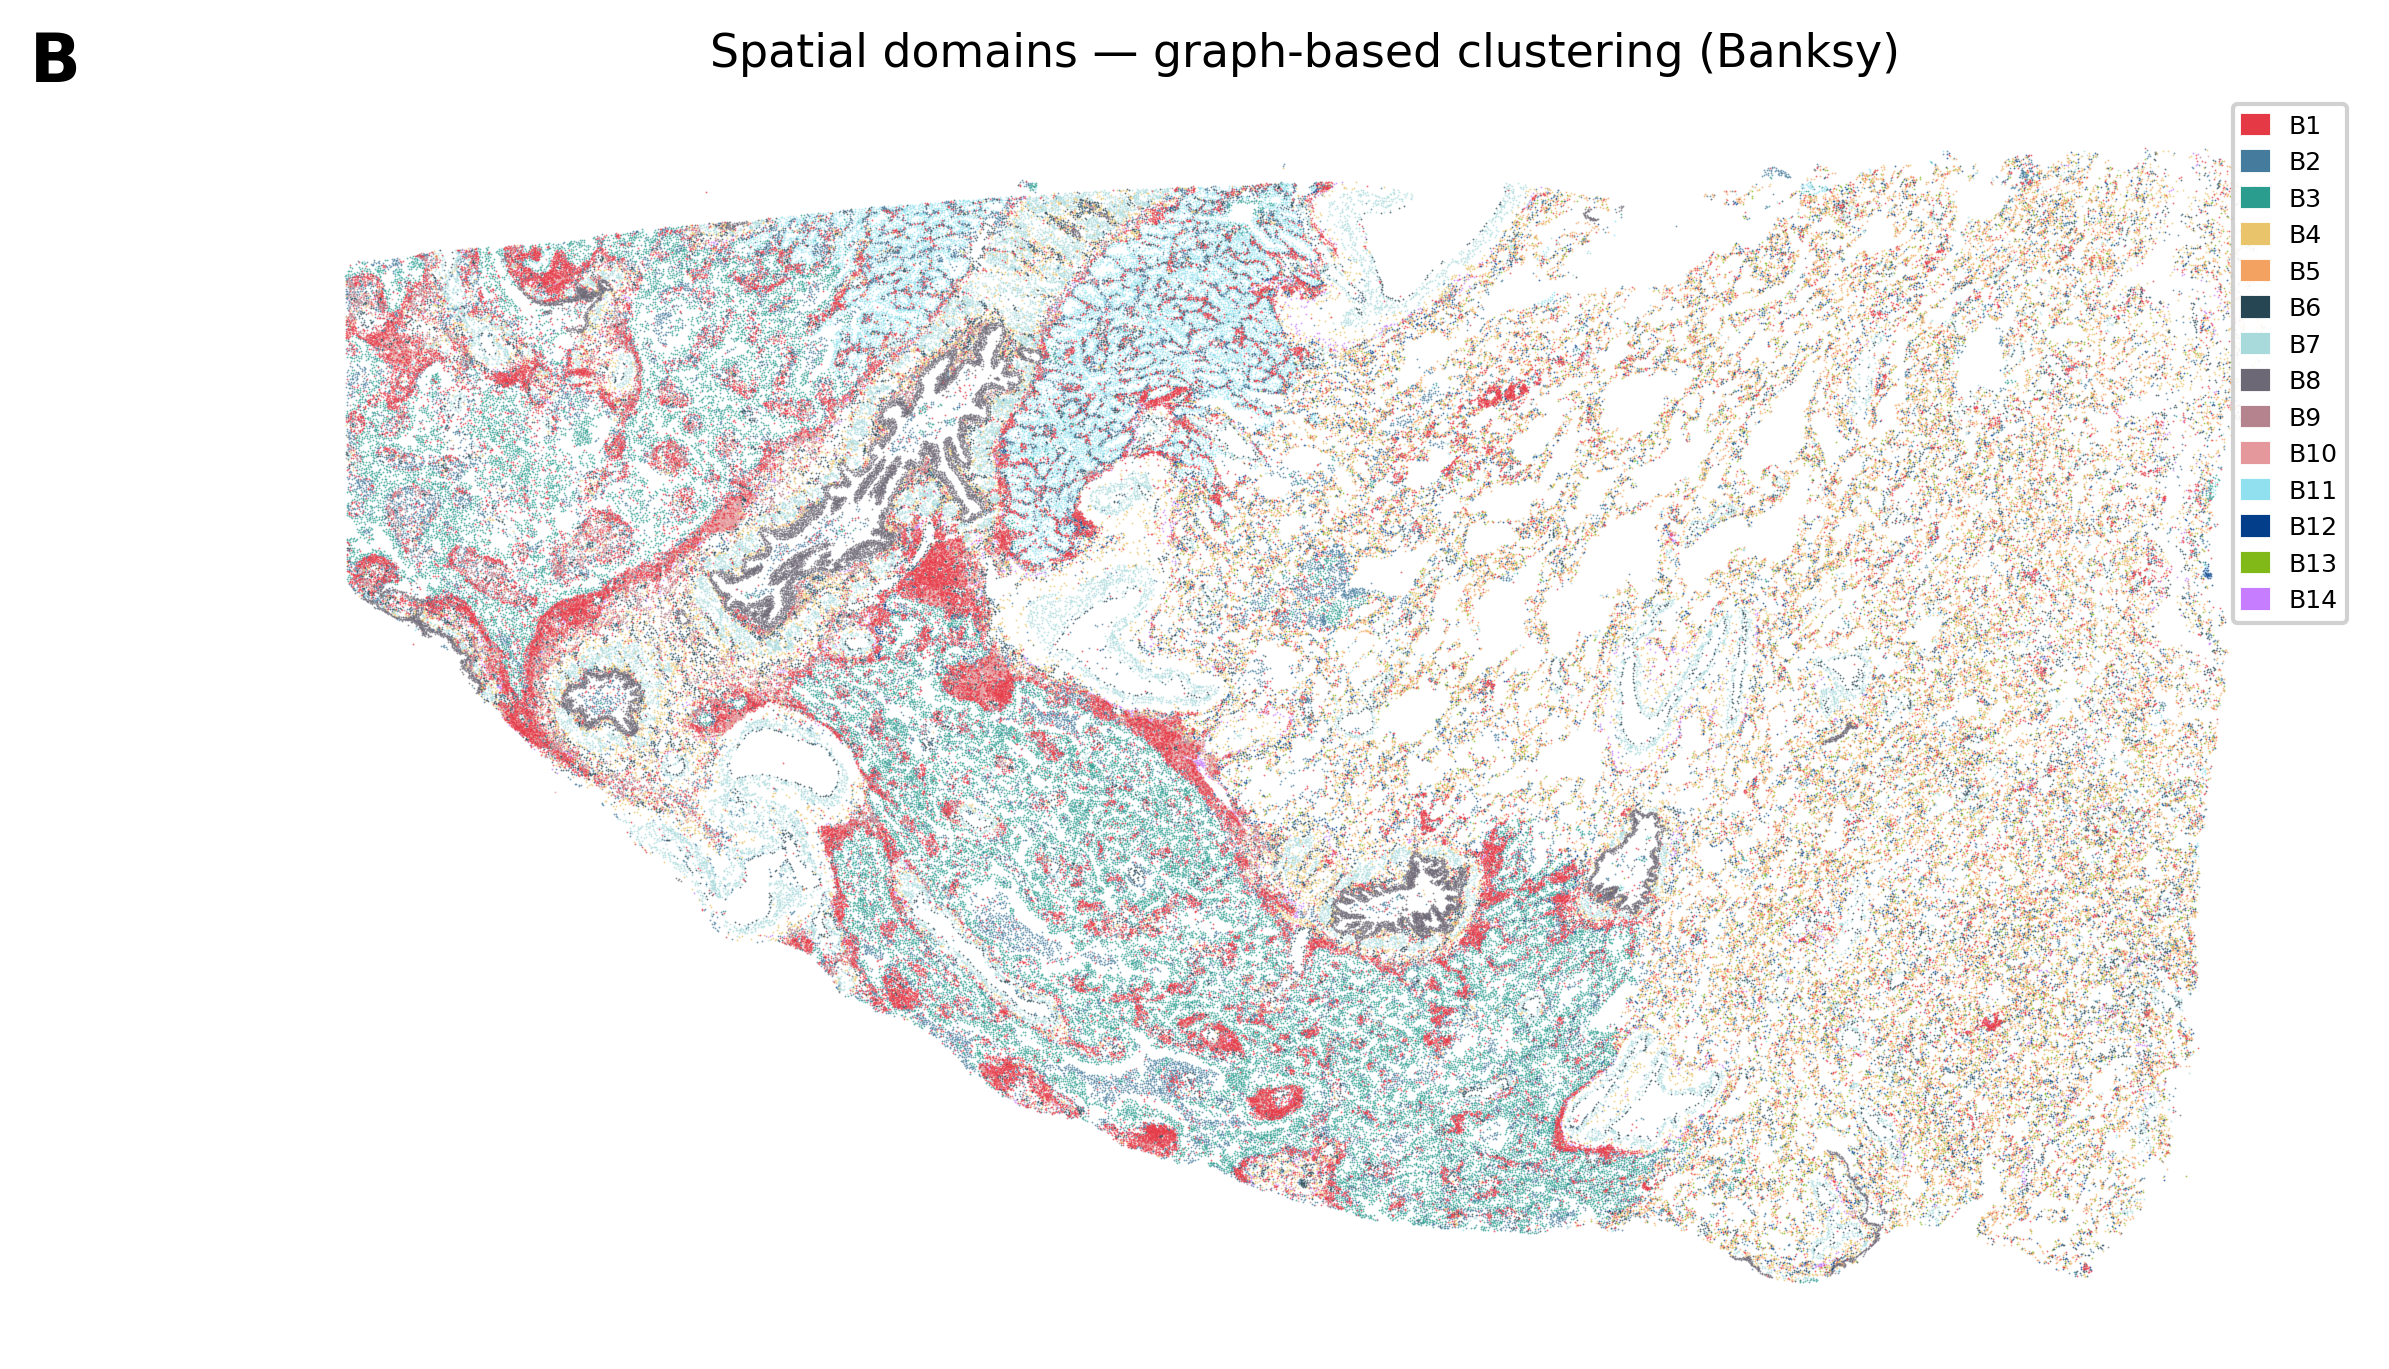
\includegraphics[width=\textwidth]{figures/Fig3B_banksy_domains.png}
  \caption{Banksy domains}
  \label{fig:3b}
\end{subfigure}
\hfill
\begin{subfigure}[b]{0.32\textwidth}
  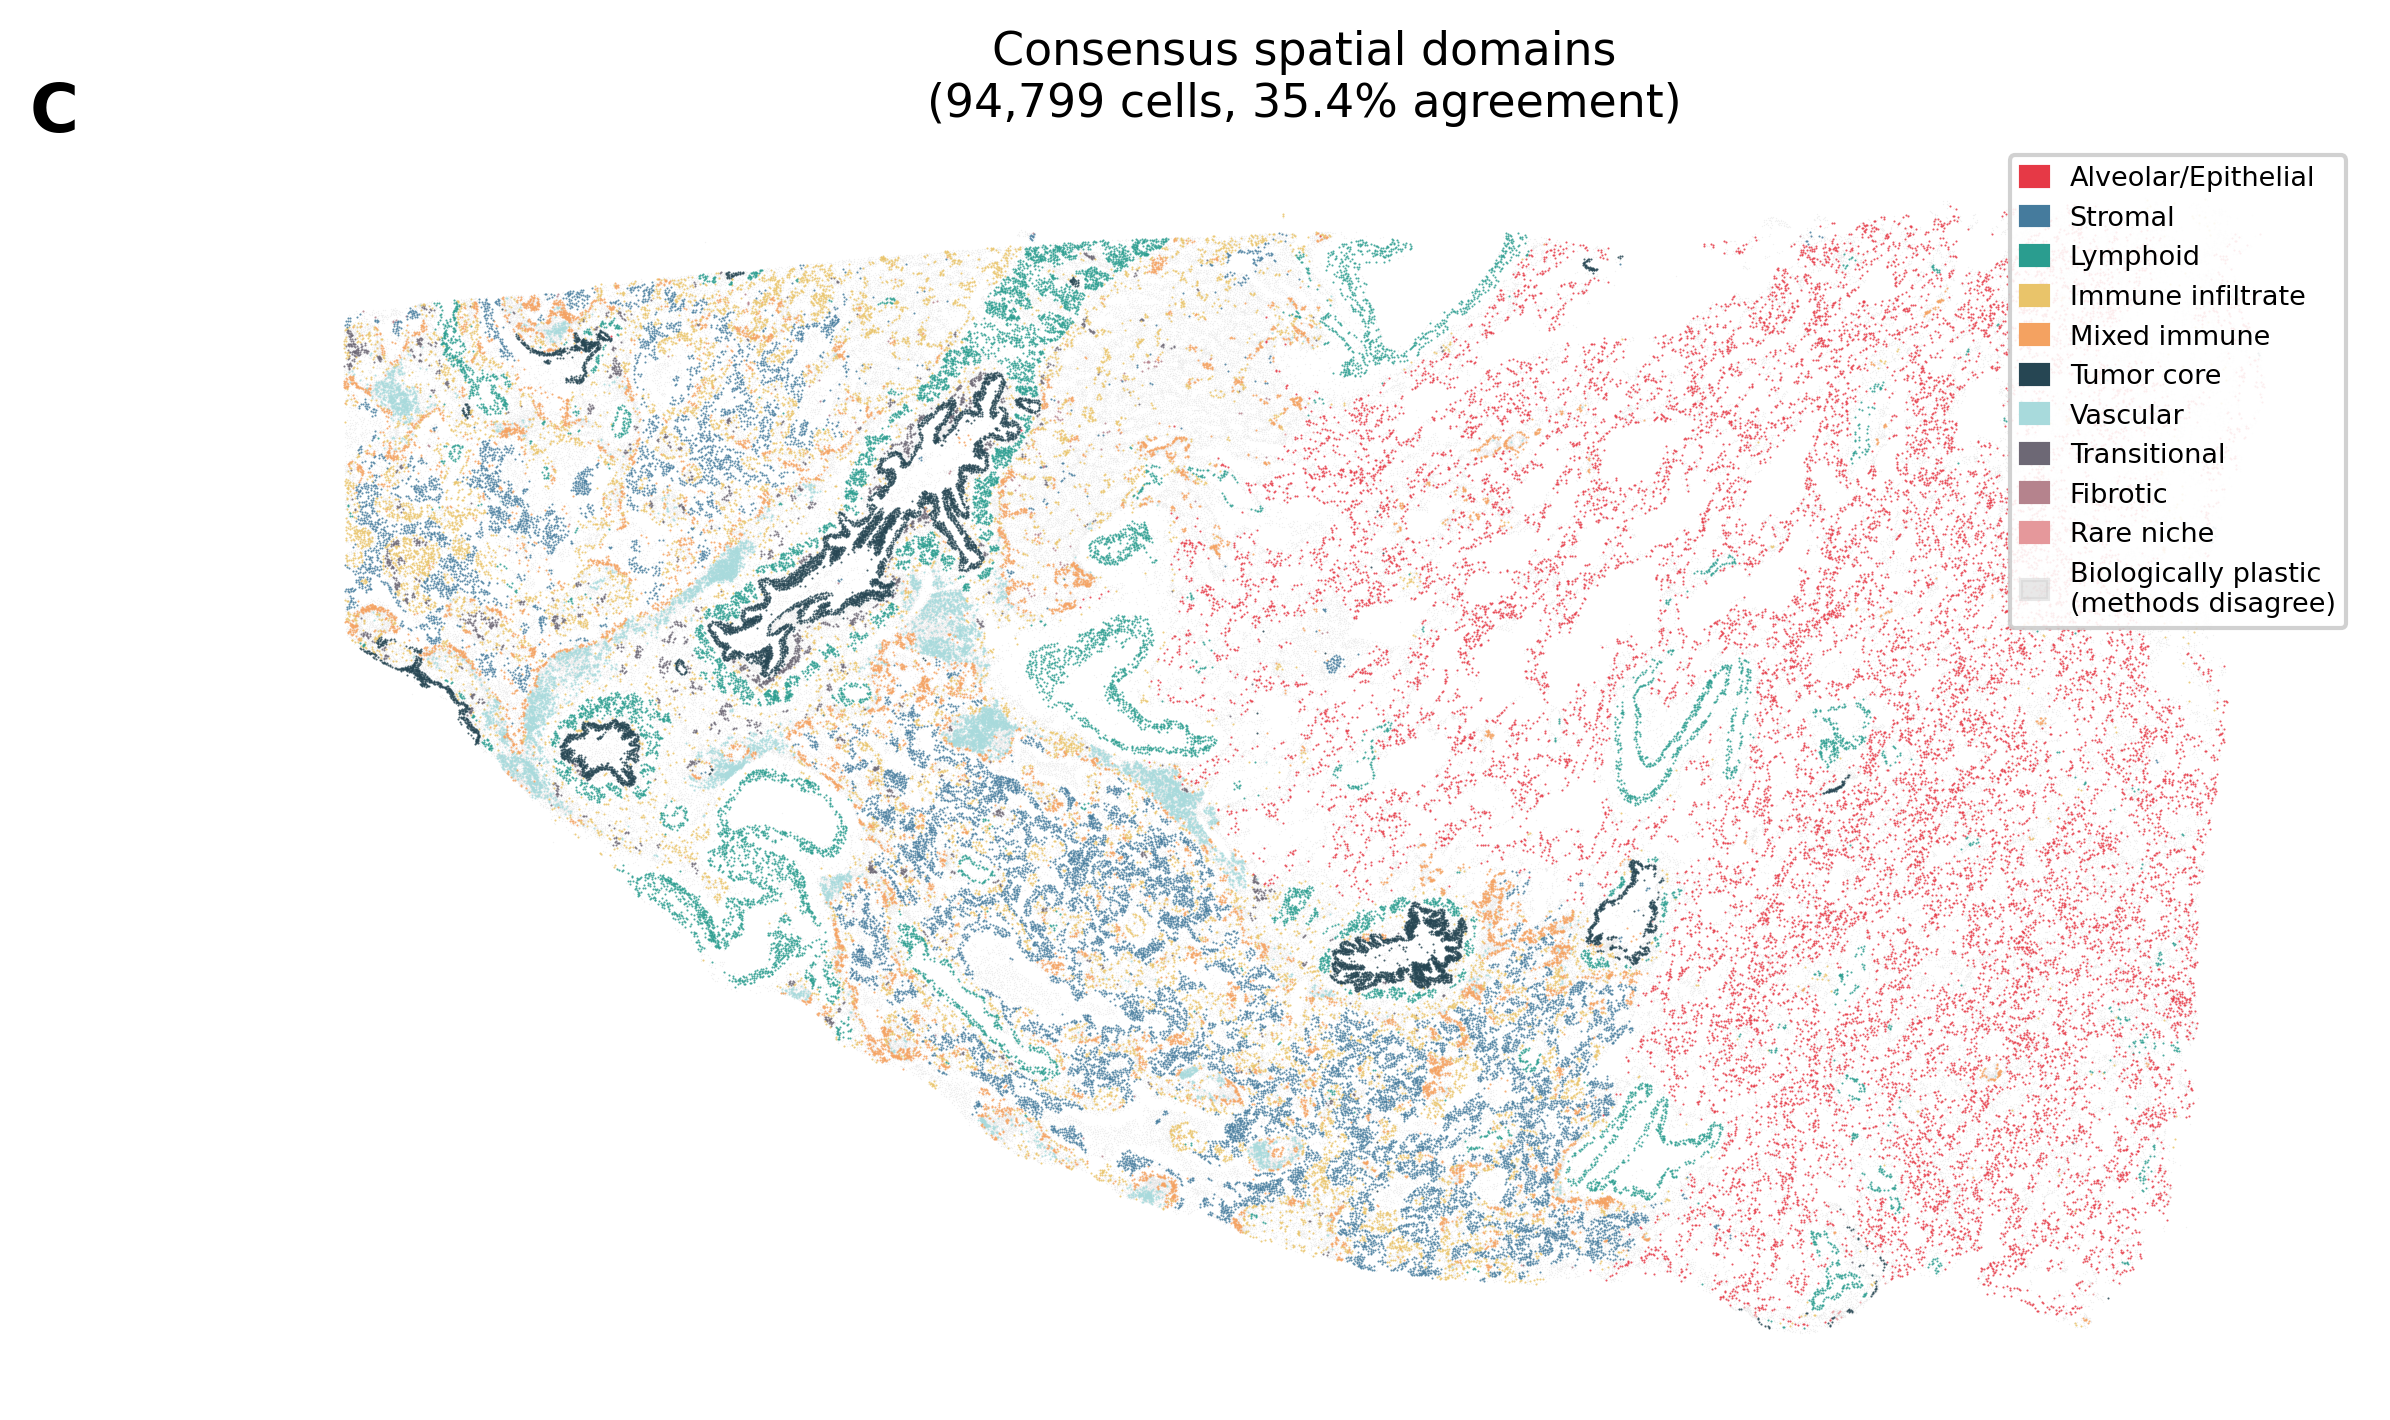
\includegraphics[width=\textwidth]{figures/Fig3C_consensus_domains.png}
  \caption{Consensus}
  \label{fig:3c}
\end{subfigure}
\caption{\textbf{Spatial domain inference by two independent methods.}
\textbf{(A)} Novae foundation-model domains (14 domains; 64-dimensional embeddings).
\textbf{(B)} Banksy graph-based domains (14 domains; $\lambda = 0.2$, $k_{\text{geom}} = 6$).
\textbf{(C)} Consensus spatial assignment: cells where both methods agree (35.4\% of cells, shown in color; non-consensus cells in gray). Consensus cells cluster in tissue compartment cores rather than boundaries.}
\label{fig:3}
\end{figure}

\subsection*{3.4 Dual-validated cell--cell communication hubs}
We analyzed cell--cell communication (CCC) using a dual-validation strategy that required independent confirmation at two computational levels: ligand--receptor scoring and spatial co-localization. In the first stage, we applied LIANA+ \citep{ramirez2024liana} with the \texttt{rank\_aggregate} method, which combines evidence from five independent CCC scoring algorithms (CellChat \citep{jin2021inference}, CellPhoneDB \citep{efremova2020cellphonedb}, NATMI \citep{hou2020predicting}, Connectome, and scSeqComm). Analyses were run with 1,000 permutations, a spatial interaction radius of 200~$\mu$m, and cosine bivariate weighting to account for spatial proximity. This yielded 2,631 interaction pairs, of which 1,565 were statistically significant at a false discovery rate of 5\%.

In the second stage, the top 30 interactions by consensus rank were submitted to Spacia \citep{zhu2024spacia}, a Bayesian multiple instance learning framework that independently evaluates whether ligand-expressing sender cells and receptor-expressing receiver cells co-localize at spatial scales finer than the LIANA+ radius. Spacia uses Markov chain Monte Carlo sampling (5,000 iterations) to estimate sender--receiver spatial betas and associated $p$-values without relying on the same ligand--receptor database as LIANA+. An interaction was declared spatially validated if it reached $p_{\text{adj}} < 0.05$ in both methods. Five interactions involving rare sender cell types ($< 500$ cells: plasma cells, plasmablasts, mature dendritic cells, and one plasmacytoid dendritic cell interaction) were excluded from Spacia analysis due to insufficient sample size for Bayesian inference, leaving 25 testable interactions.

Of these 25, 22 (88\%) were confirmed by both methods, demonstrating that the majority of LIANA+ predictions reflect genuine spatial proximity rather than statistical artifacts of the ligand--receptor scoring framework (Figure~\ref{fig:4}). The three non-validated interactions involved low-abundance sender cell types at the detection limit of the 289-gene panel.

The dominant validated hub involves the ADAM17 ligand and MUC1 receptor (Figure~\ref{fig:4}). ADAM17 is a metalloprotease that cleaves and activates multiple membrane-bound cytokines and growth factors \citep{lambrecht2018adam17}, while MUC1 is an oncogenic mucin overexpressed on tumor epithelial cells and involved in immune evasion \citep{nath2013muc1}. In our data, ADAM17--MUC1 signaling originates from seven distinct sender cell types --- alveolar type 1 cells, M1-like and M2-like macrophages, classical monocytes, pericytes, cDC1, and cDC2 --- all converging on tumor resting cells as the primary receiver, with adjusted $p$-values ranging from $4.1 \times 10^{-12}$ to $1.1 \times 10^{-71}$. The activation of this axis in both M1-like and M2-like macrophages suggests that it operates independently of macrophage polarization state, implicating ADAM17--MUC1 as a non-canonical, shedding-mediated immunosuppressive mechanism complementary to the PD-1/PD-L1 checkpoint axis. Two additional validated axes --- LTF--AGER (tumor cells toward alveolar type 1) and S100B--AGER (dendritic cells toward alveolar type 1) --- point to tumor-driven invasion of the alveolar niche as a secondary signaling theme.

\begin{figure}[htbp]
\centering
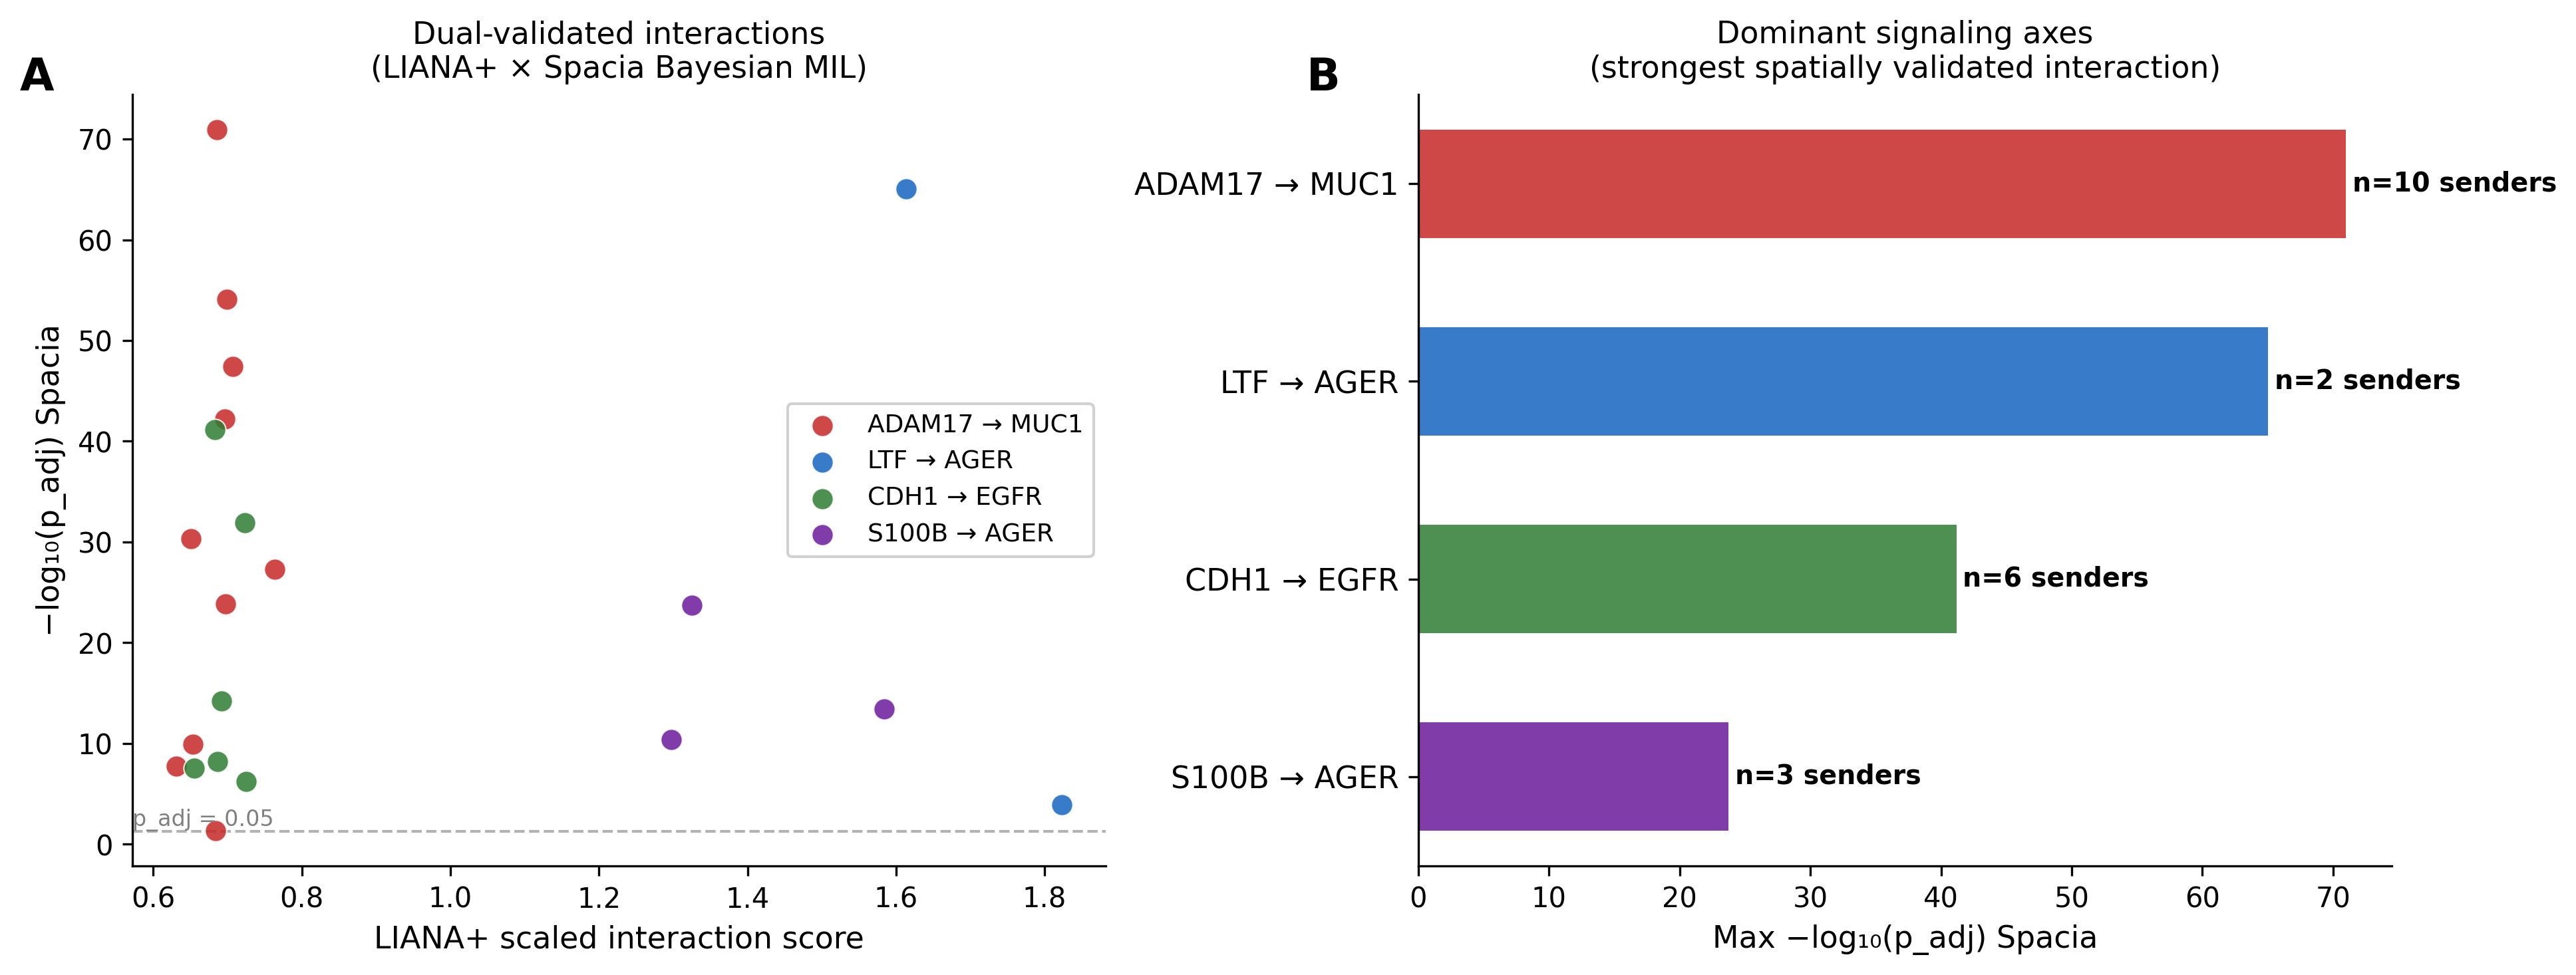
\includegraphics[width=0.85\textwidth]{figures/Fig4B_spacia_axes.png}
\caption{\textbf{Spatially validated cell--cell communication hubs.}
Bar chart showing the top dual-validated ligand--receptor interactions, ranked by Spacia adjusted $p$-value. Color indicates the sender cell type; bar length represents $-\log_{10}(p_{\text{adj}})$. The ADAM17--MUC1 axis (orange, multiple senders) dominates the validated interaction landscape. All 22 interactions shown reached significance in both LIANA+ rank\_aggregate ($n=5$ methods, 1,000 permutations) and Spacia Bayesian spatial inference ($p_{\text{adj}} < 0.05$).}
\label{fig:4}
\end{figure}

\subsection*{3.5 Spatial pseudotime reveals TME gradient}
To characterize the developmental and compositional dynamics of the TME along a continuous axis from healthy parenchyma toward the tumor core, we constructed spatial pseudotime trajectories using Slingshot \citep{street2018slingshot} applied to Novae 64-dimensional latent embeddings. Novae embeddings were chosen as the trajectory input because they integrate both transcriptional state and spatial context, producing a representation that is better suited to spatial trajectory inference than conventional principal component-based embeddings \citep{schaar2025novae}. Trajectories were computed on a stratified subsample of 29,991 cells that preserved cell-type proportions across the tissue, with the centroid of proliferating tumor cells designated as the root state (pseudotime = 0).

Slingshot inferred eight principal curve lineages from the data manifold, each representing a distinct cellular transition pathway. Lineage 1, the primary trajectory, contains 17,612 cells and spans a gradient from resting alveolar cells through macrophage-enriched intermediates to tumor epithelial populations. We subsequently applied generalized additive models (GAMs) via tradeSeq \citep{vandenberge2020tradeseq} to the Novae dimensions along Lineage 1, identifying transcriptional and neighborhood-compositional transitions that are statistically significant after correction for multiple testing.

Visualization of cell-type proportions across 20 equally spaced pseudotime bins along Lineage 1 reveals a striking compositional gradient (Figure~\ref{fig:5}). Early pseudotime bins (healthy parenchyma) are dominated by alveolar type 1 and type 2 cells, with sparse immune infiltration. As pseudotime increases toward the tumor, there is a monotonic enrichment of M2-like macrophages and classical monocytes, peaking at intermediate pseudotime values, followed by a final transition dominated by tumor epithelial cells. Dendritic cell subsets --- particularly cDC1 and cDC2 --- show a transient enrichment at intermediate pseudotime, consistent with antigen-presenting roles at the tumor--parenchyma boundary. Notably, T cells and NK cells remain at low proportions throughout the trajectory, suggesting that cytotoxic immune activity is numerically suppressed or spatially excluded from the dominant transition axis, in agreement with the immunosuppressive architecture inferred from the cell--cell communication analysis.

The temporal ordering imposed by pseudotime thus provides a complementary perspective to the static spatial domain map: the same myeloid-dominated immunosuppressive niche identified by spatial domain analysis is recapitulated as the dominant intermediate state in the major TME transition trajectory. This convergence of evidence from three independent analytical frameworks --- domain inference, communication validation, and pseudotime --- reinforces the biological robustness of the myeloid immunosuppression model.

\begin{figure}[htbp]
\centering
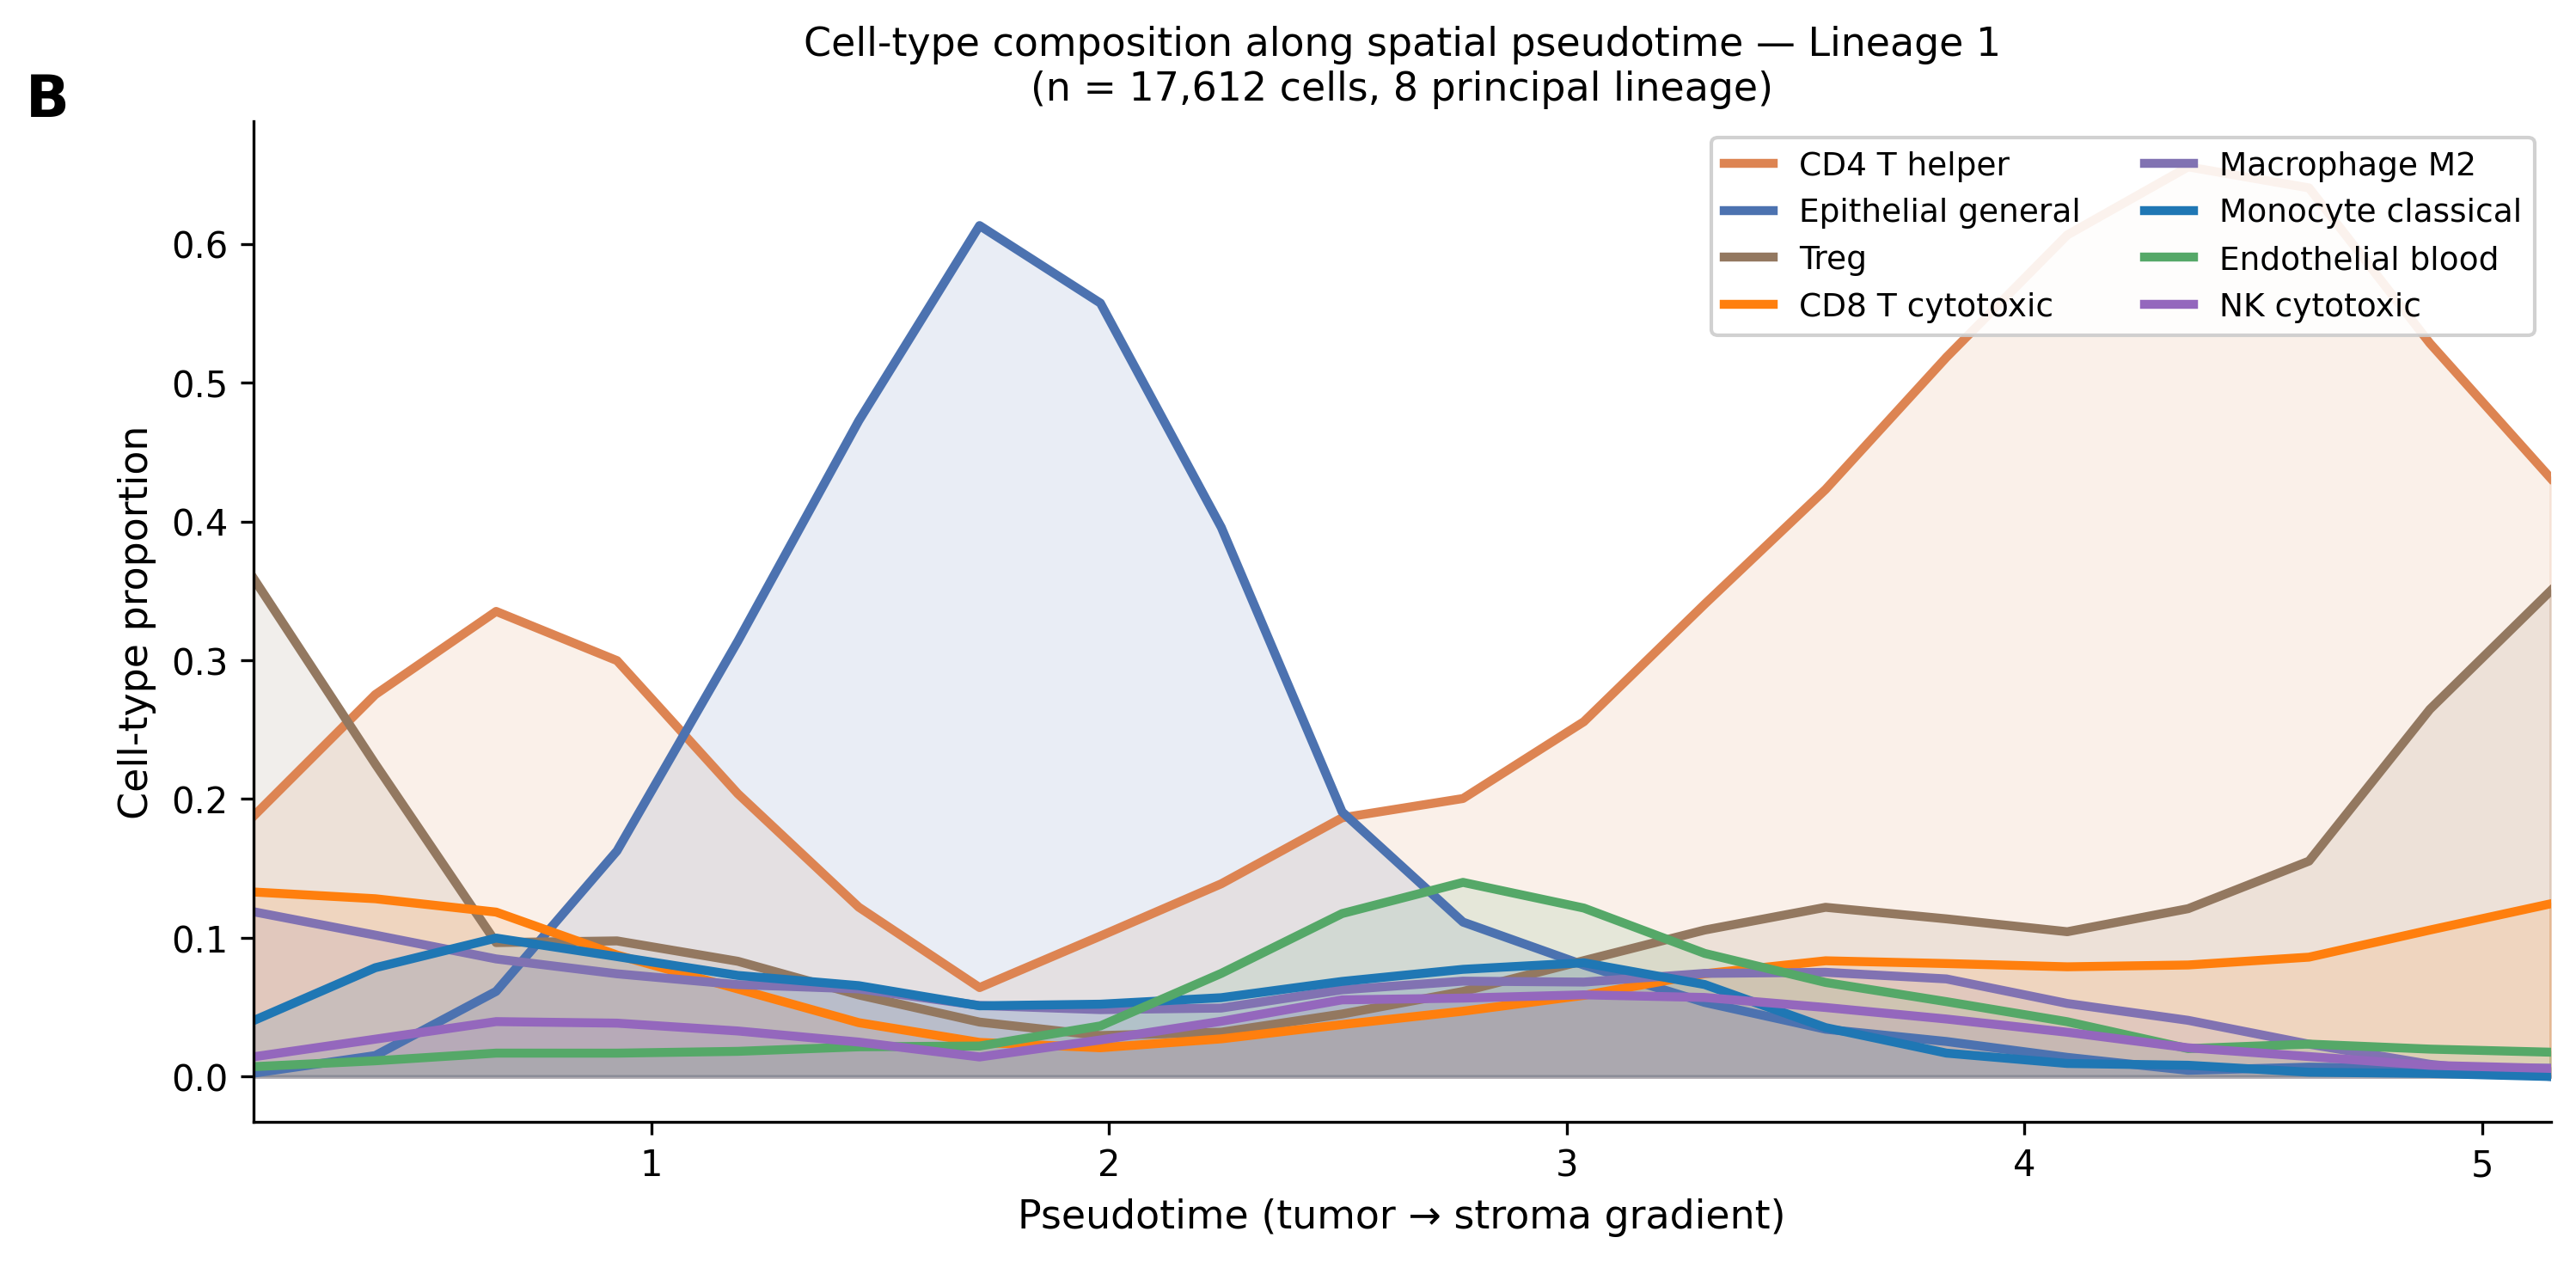
\includegraphics[width=0.85\textwidth]{figures/Fig5B_pseudotime_proportions.png}
\caption{\textbf{Cell-type compositional dynamics along the primary TME pseudotime trajectory.}
Stacked area chart showing cell-type proportions across 20 pseudotime bins along Lineage 1 (17,612 cells; root = proliferating tumor cells, terminal = alveolar parenchyma). M2-like macrophages and classical monocytes dominate intermediate pseudotime, consistent with a myeloid-enriched immunosuppressive transition zone between healthy alveolar tissue (right) and the tumor core (left). T cells and NK cells remain at consistently low proportions throughout the trajectory.}
\label{fig:5}
\end{figure}

\section*{Discussion}
\label{sec:discussion}

We present a multi-tool consensus framework for \textit{in situ} spatial transcriptomics and demonstrate its application to human lung adenocarcinoma. The central methodological principle --- retaining only findings confirmed by at least two independent computational tools per analytical family --- substantially reduces the risk of reporting tool-specific artifacts as biological findings. The 88\% validation rate of LIANA+ interactions by independent Bayesian spatial inference, and the 99.7\% consensus SVG rate across three autocorrelation methods, suggest that targeted spatial transcriptomics panels carry sufficient signal for robust analytical conclusions when multiple methods are applied in parallel.

The most prominent biological finding is the ADAM17--MUC1 signaling hub. ADAM17 (also known as TACE) is a sheddase that processes ectodomains of TNF-$\alpha$, TGF-$\alpha$, EGF-R ligands, and multiple other substrates \citep{lambrecht2018adam17}. Its activity in myeloid cells --- particularly macrophages --- has been linked to immunosuppressive cytokine release and tumor-promoting stromal remodeling. MUC1, the receiver, is an oncomucin whose intracellular domain activates NF-$\kappa$B and Wnt signaling in tumor cells and whose extracellular domain physically blocks immune effector binding \citep{nath2013muc1}. Our data reveal that this axis is active across both M1-like and M2-like macrophage states, suggesting it is not dependent on a specific polarization context but instead represents a constitutive feature of the myeloid--tumor cell interface. This finding extends existing in vitro evidence for ADAM17--MUC1 co-activity to intact FFPE spatial tissue and motivates therapeutic evaluation of ADAM17 inhibitors in combination with checkpoint agents.

The spatial domain and pseudotime analyses converge on a consistent anatomical motif: a myeloid-enriched intermediate zone between healthy alveolar parenchyma and the tumor core. This spatial arrangement is distinct from the immune desert or inflamed TME archetypes defined in bulk transcriptomics \citep{chen2016elements}. The enrichment of M2-like macrophages and monocytes at the tumor margin, rather than T cells or NK cells, identifies this sample as an immune-excluded or myeloid-suppressed TME, which is associated with poor prognosis and reduced checkpoint immunotherapy response in lung adenocarcinoma \citep{cassetta2020targeting, wu2021single}.

Several limitations of this study warrant discussion. First, the 289-gene Xenium panel precluded analysis of transcription factors, non-coding RNAs, and many immune checkpoints not included in the standard lung expression panel; whole-transcriptome spatial methods such as Visium HD or MERFISH would be required to address these gaps. Second, the analysis is based on a single tissue section from one patient, and whether the ADAM17--MUC1 hub and myeloid spatial organization are generalizable across lung adenocarcinoma subtypes and stages requires validation in larger cohorts. Third, FFPE tissue chemistry introduces transcript fragmentation that may affect detection of low-abundance transcripts; however, the concordance of spatially variable gene findings across three independent methods suggests that this technical artifact did not substantially affect our conclusions.

Future work will apply this consensus pipeline to Xenium liver tissue data, where larger gene panels will enable resolution of rare hepatic stellate cell and Kupffer cell subpopulations. The framework is designed to scale: each analytical module is implemented as an independent workflow rule, allowing plug-and-play replacement of individual tools as the field advances.

\section*{Methods}
\label{sec:methods}

\subsection*{Dataset and preprocessing}
We analyzed a publicly available Xenium \textit{in situ} dataset of human lung adenocarcinoma (10x Genomics, accession CG000709 Rev C). The tissue was obtained from an FFPE block (Avaden Biosciences) of a Stage IB invasive acinar adenocarcinoma (T2a N0 MX). Gene expression profiling used the Xenium Human Lung Gene Expression Panel v1.1 (289 target genes plus 87 negative control probes). Xenium Onboard Analysis v3.0.0 was run on the instrument to produce cell segmentation and transcript assignment outputs.

Quality control was applied to remove cells with fewer than 5 transcripts, cell area greater than 1,500~$\mu$m$^{2}$, and negative control probes. A total of 268,034 cells passed filtering from 278,659 detected (96.2\% retention rate). Transcript counts were normalized using \texttt{scanpy} \citep{wolf2018scanpy}: library-size normalization to 10,000 counts per cell, followed by $\log_{1p}$ transformation. Raw counts were retained in a separate layer for tools requiring integer input. All data were stored in the SpatialData Zarr format using \texttt{spatialdata} \citep{marconato2024spatialdata}.

\subsection*{Cell-type annotation}
Cell-type annotation followed a three-source hybrid strategy. First, immune cells were identified by iterative subclustering: broad immune populations were isolated by expression of canonical markers available in the panel, then reclustered at higher resolution to resolve myeloid and lymphoid subtypes. Second, all 268,034 cells underwent Leiden community detection at multiple resolutions ($\gamma = 0.3$, $0.5$, $0.8$) on a shared nearest-neighbor graph built from the top 30 principal components of log-normalized expression, and community labels were assigned to the highest-scoring known cell type using \texttt{scanpy.tl.score\_genes}. Third, a scoring approach using curated gene signatures (3--12 marker genes per type derived from published lung and immune cell atlases \citep{travaglini2020molecular}) resolved ambiguous cells. Cells scoring below threshold in all signatures were labelled Unassigned (4.8\% of cells). The final taxonomy comprises 14 broad categories, 26 granular subtypes, and 7 functional states. Annotation concordance was assessed by computing the adjusted Rand index (ARI) between the primary annotation and an independent computational subclustering of immune cells, yielding ARI = 0.742.

\subsection*{Spatially variable gene identification}
Three methods were applied to identify spatially variable genes (SVGs). Hotspot \citep{detomaso2021hotspot} v1.0.0 computed local autocorrelation statistics for each gene using a Gaussian kernel neighborhood model; genes with $Z$-score $> 1.96$ were retained. nnSVG \citep{weber2023nnsvg} v1.2 fitted rank-based non-parametric Gaussian process models on a random subsample of 10,000 cells (seed = 42); genes with FDR $< 0.05$ were retained. Moran's~I was computed using \texttt{squidpy.gr.spatial\_autocorr} \citep{palla2022squidpy} on a $k$-nearest-neighbor graph ($k=6$); genes with corrected $p < 0.05$ (Benjamini--Hochberg) were retained. A gene was declared a consensus SVG if significant in at least two of three methods. All 289 genes were tested; 288 (99.7\%) met the consensus criterion.

\subsection*{Spatial domain inference}
Spatial domain inference used two independent approaches. Novae \citep{schaar2025novae} (model: novae-human-0, MICS-Lab) was applied with default hyperparameters, producing 64-dimensional latent embeddings per cell. Embeddings were clustered at multiple resolutions; 14 domains were selected based on biological interpretability and silhouette score. Banksy \citep{zhao2023banksy} was run with neighborhood aggregation parameter $\lambda = 0.2$, geometric neighborhood $k_{\text{geom}} = 6$, and Leiden community detection at $\gamma = 0.5$, yielding 14 domains. Consensus domain assignment was defined as cells where both methods independently assigned the same domain label; 94,869 cells (35.4\%) met this criterion.

\subsection*{Cell--cell communication analysis}
Cell--cell communication was analyzed in two stages. First, LIANA+ \citep{ramirez2024liana} v1.7.1 was run using the \texttt{rank\_aggregate} consensus method, which aggregates $p$-values and ranks from CellChat \citep{jin2021inference}, CellPhoneDB \citep{efremova2020cellphonedb}, NATMI \citep{hou2020predicting}, Connectome, and scSeqComm. Analysis used 1,000 permutations, a spatial radius of 200~$\mu$m, and cosine bivariate spatial weighting to account for cell proximity. The top 30 interactions by consensus rank were selected for the second stage.

Second, Spacia \citep{zhu2024spacia} was applied to each of the 30 candidate interactions using the full spatial coordinates and per-cell normalized expression. Spacia employs Bayesian multiple instance learning with MCMC sampling (5,000 iterations, 2,500 burn-in) to estimate whether the spatial arrangement of sender--receiver cell pairs is consistent with directional signaling. Sender cell types with fewer than 500 cells were excluded (5 interactions), leaving 25 testable pairs. An interaction was considered dual-validated if LIANA+ rank\_aggregate $p_{\text{adj}} < 0.05$ \textit{and} Spacia $p_{\text{adj}} < 0.05$. Of 25 tested interactions, 22 (88\%) met both criteria.

\subsection*{Spatial pseudotime analysis}
Pseudotime trajectory inference used the Novae 64-dimensional embeddings for a stratified subsample of 29,991 cells (cell-type-proportional sampling, seed = 42). Slingshot \citep{street2018slingshot} v2.6 was run in R (v4.3.3) using the \texttt{slingshot} Bioconductor package, with the centroid of the proliferating tumor cell cluster designated as the root state. Eight principal curve lineages were inferred. Generalized additive models along Lineage 1 (17,612 cells) were fitted using tradeSeq \citep{vandenberge2020tradeseq} v1.12 with $k = 6$ knots per spline; significance was assessed by the association test with Bonferroni correction. For visualization, cells were assigned to 20 equally spaced pseudotime bins and cell-type proportions were computed per bin.

\subsection*{Software and reproducibility}
All Python analyses were run in a dedicated conda environment containing spatialdata 0.2, scanpy 1.9, liana 1.7.1, novae 0.3, hotspotsc 1.0, and Banksy 0.1.9. R analyses used a separate conda environment with Bioconductor 3.18: slingshot 2.6, tradeSeq 1.12, nnSVG 1.5, and Banksy 1.0 (R implementation). Spacia was run in a dedicated Python 3.8 environment with R 4.5.3. All workflows are implemented as Snakemake \citep{molder2021snakemake} rules with environment-locked YAML files. Figures were generated using matplotlib \citep{hunter2007matplotlib}, seaborn, and Crameri perceptually uniform colormaps \citep{crameri2023scientific}. Analysis code is available at [GitHub repository pending]. The dataset is publicly available at the 10x Genomics website (CG000709 Rev C).

\section*{Data availability}
The dataset analyzed in this study is publicly available from the 10x Genomics website under accession CG000709 Rev C.

\section*{Code availability}
All analysis scripts are available at [GitHub repository --- link pending upon acceptance].

\section*{Acknowledgements}
We thank the Instituto Nacional de Pediatr\'{i}a and the Instituto de Investigaciones Biom\'{e}dicas (UNAM) for providing institutional resources and computational infrastructure. Funding information: pending.

\section*{Author contributions}
M.A.D.-C.: Conceptualization, Methodology, Software, Formal analysis, Data curation, Writing -- original draft. A.R.G.: Supervision, Writing -- review \& editing, Funding acquisition, Resources.

\section*{Competing interests}
The authors declare no competing interests.

\bibliographystyle{unsrtnat}
\bibliography{refs}

%% ===== SUPPLEMENTARY =====
\newpage
\setcounter{section}{0}
\renewcommand{\thesection}{S\arabic{section}}
\renewcommand{\thefigure}{S\arabic{figure}}
\setcounter{figure}{0}
\section*{Supplementary Information}

\subsection*{Supplementary Figure 1 --- Quality control metrics}
\begin{figure}[h!]
\centering
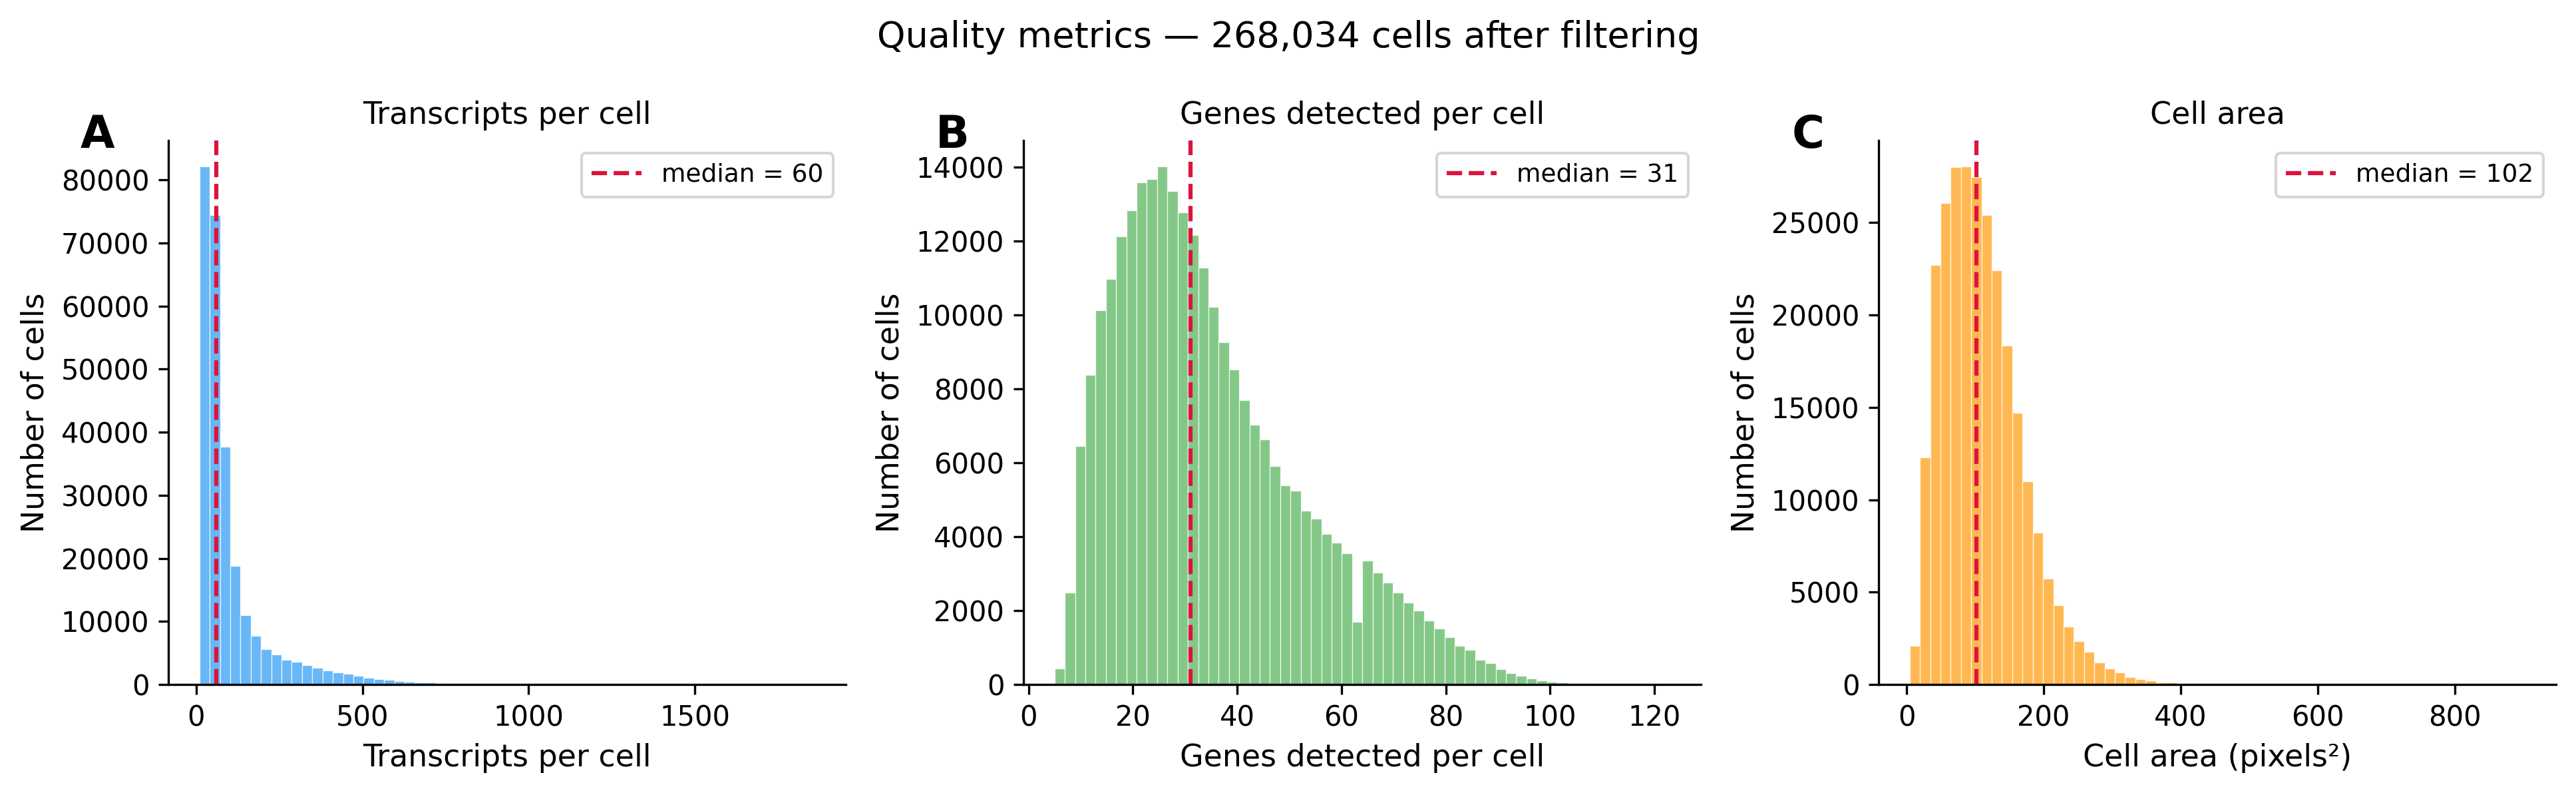
\includegraphics[width=\textwidth]{figures/FigS1_qc_metrics.png}
\caption{\textbf{Quality control metrics.} Distribution of per-cell transcript count, detected genes, and cell area before and after filtering. Thresholds applied: transcript count $\geq$5, cell area $\leq$1,500~\textmu m$^{2}$. A total of 268,034 cells passed quality control from 278,659 detected.}
\label{fig:s1}
\end{figure}

\end{document}
